\clearpage

\section{Validation of the $\bar{\nu}/\nu$ joint analysis}
\label{sec:validation}

The validation of the fit is performed first by comparing the confidence intervals, obtained
with Asimov data sets corresponding to the oscillation parameters in tab.~\ref{tab:osc_params_joint_asimov}
%as well as the Run 1-4 data, 
with the other group analyses \cite{Mach3JointFitRun16}.
Then the coverage study is performed for 1-dimensional $\delta_{CP}$ with reactor constraint fits,
in order to verify if the ``constant $\Delta \chi^2$" method is reliable or
the ``Feldman-Cousins" method is needed.
%Pull studies will be shown for 1-dimensional fits of the following oscillation parameters:
%$\delta_{CP}$, $\sin^2 \theta_{13}$, $\sin^2 \theta_{23}$ and $|\Delta m^2_{32}|$,
%for which $\pm 1 \sigma$ ranges will be quoted by using the ``constant $\Delta \chi^2$ method".
%Since the nuisance parameters are marginalised in the fit, pull studies for these parameters do not make sense
%and will not be shown.


%
% Sensitivities and comparisons with other analysis groups
%

\subsection{Sensitivity studies}
\label{sec:sensi}

The critical values of constant $\Delta \chi^2$ method
in 1-dimensional confidence intervals are given 
by $Z\sigma = \sqrt{\Delta \chi^2}$  
where $Z$ is the number of standard deviations that
defines the confidence level.
For 90\% CL the critical value is 2.71.
The critical values for 2-dimensional fits are 2.3 and 4.61
respectively for 68\% and 90\% CL.

In Fig.~\ref{fig:validation_sensi_dcp} the sensitivity to $\delta_{CP}$ 
with reactor constraint and T2K only is shown for the Asimov data sets A and B.
%and compared with the result obtained by the other analysis groups.

\begin{figure*}[htb]
\center
%
\includegraphics[width=0.9\textwidth]{./images/missing_plot-eps-converted-to.pdf}
%
\includegraphics[width=0.9\textwidth]{./images/missing_plot-eps-converted-to.pdf}
\begin{subfigure}[b]{0.49\textwidth}
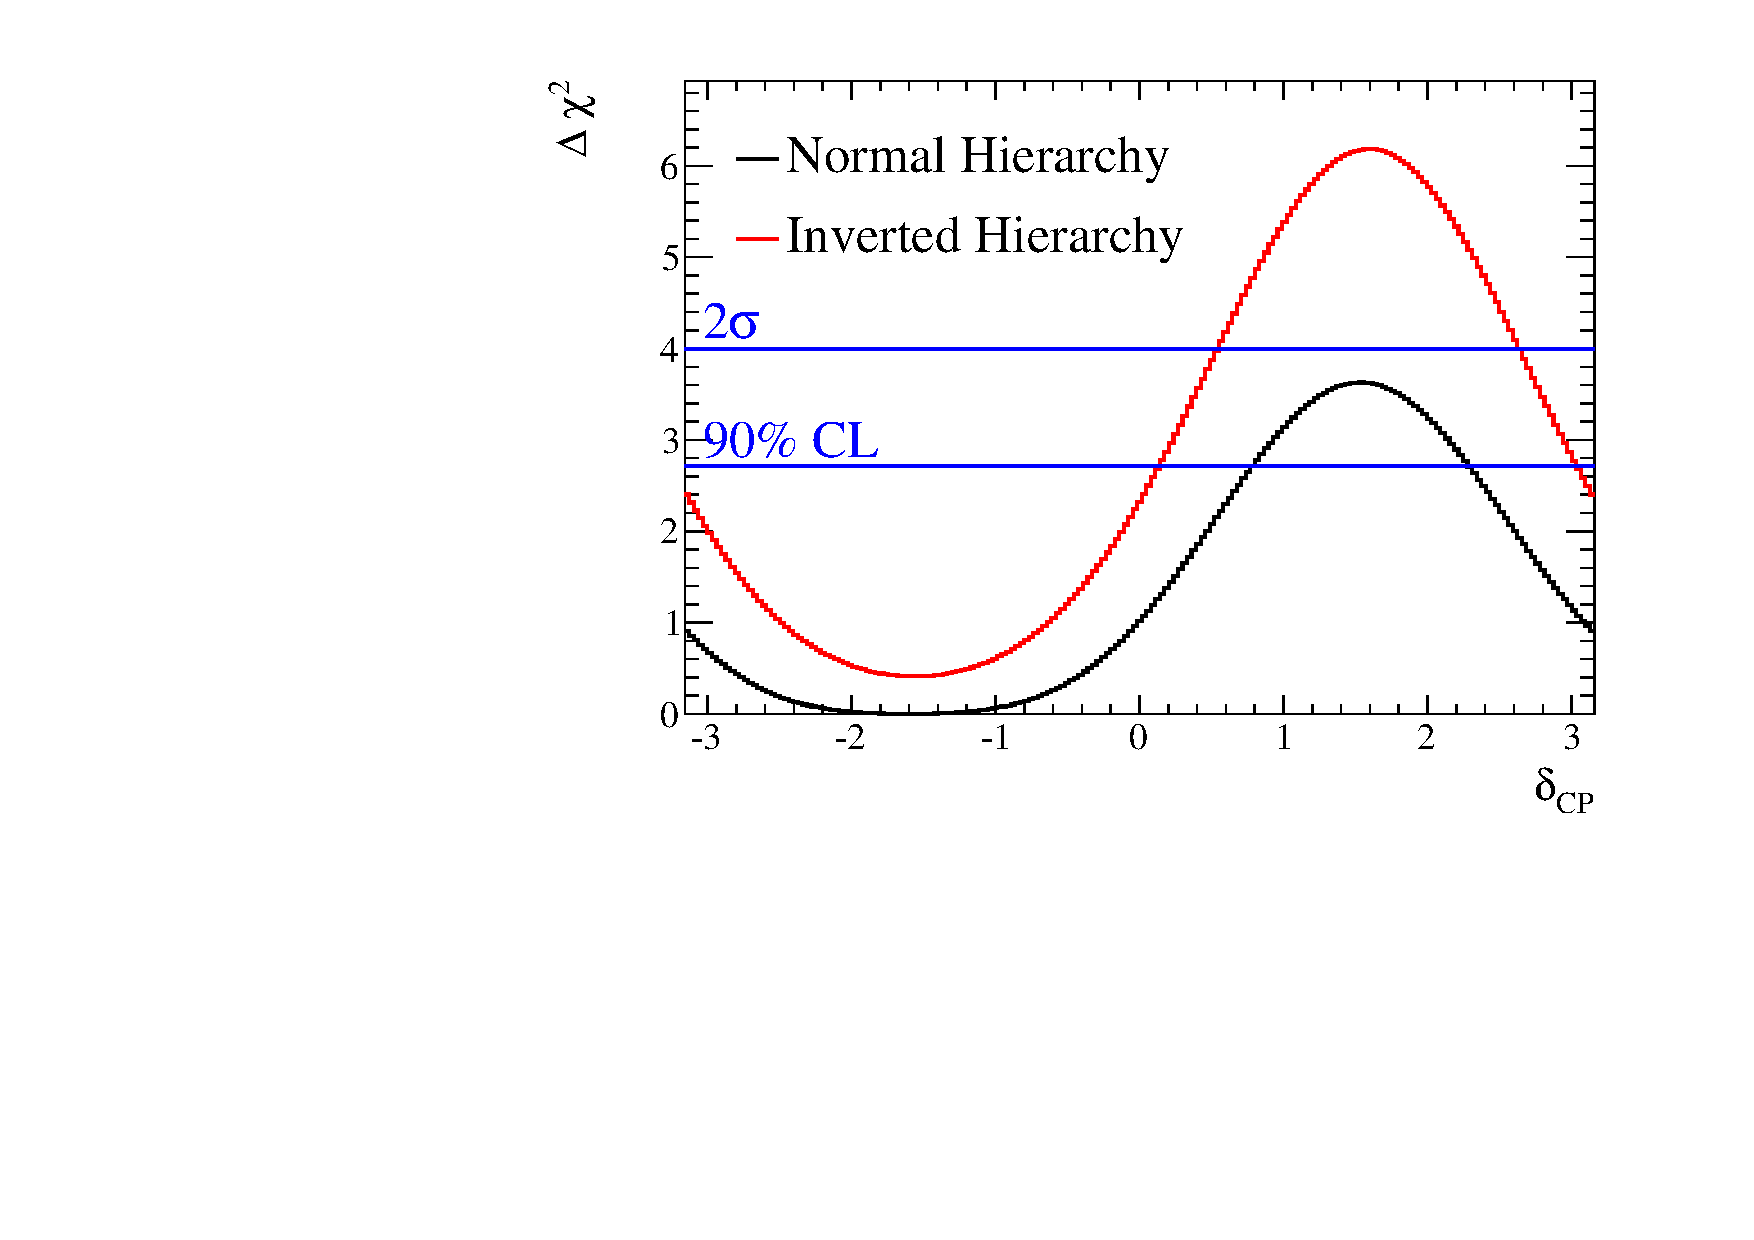
\includegraphics[width=0.9\textwidth]{./joint_plots/sensitivities/dcp_1D/dcp_react_Asimov_A.pdf}
\caption{Asimov A: with reactor constraint}
\end{subfigure}
\begin{subfigure}[b]{0.49\textwidth}
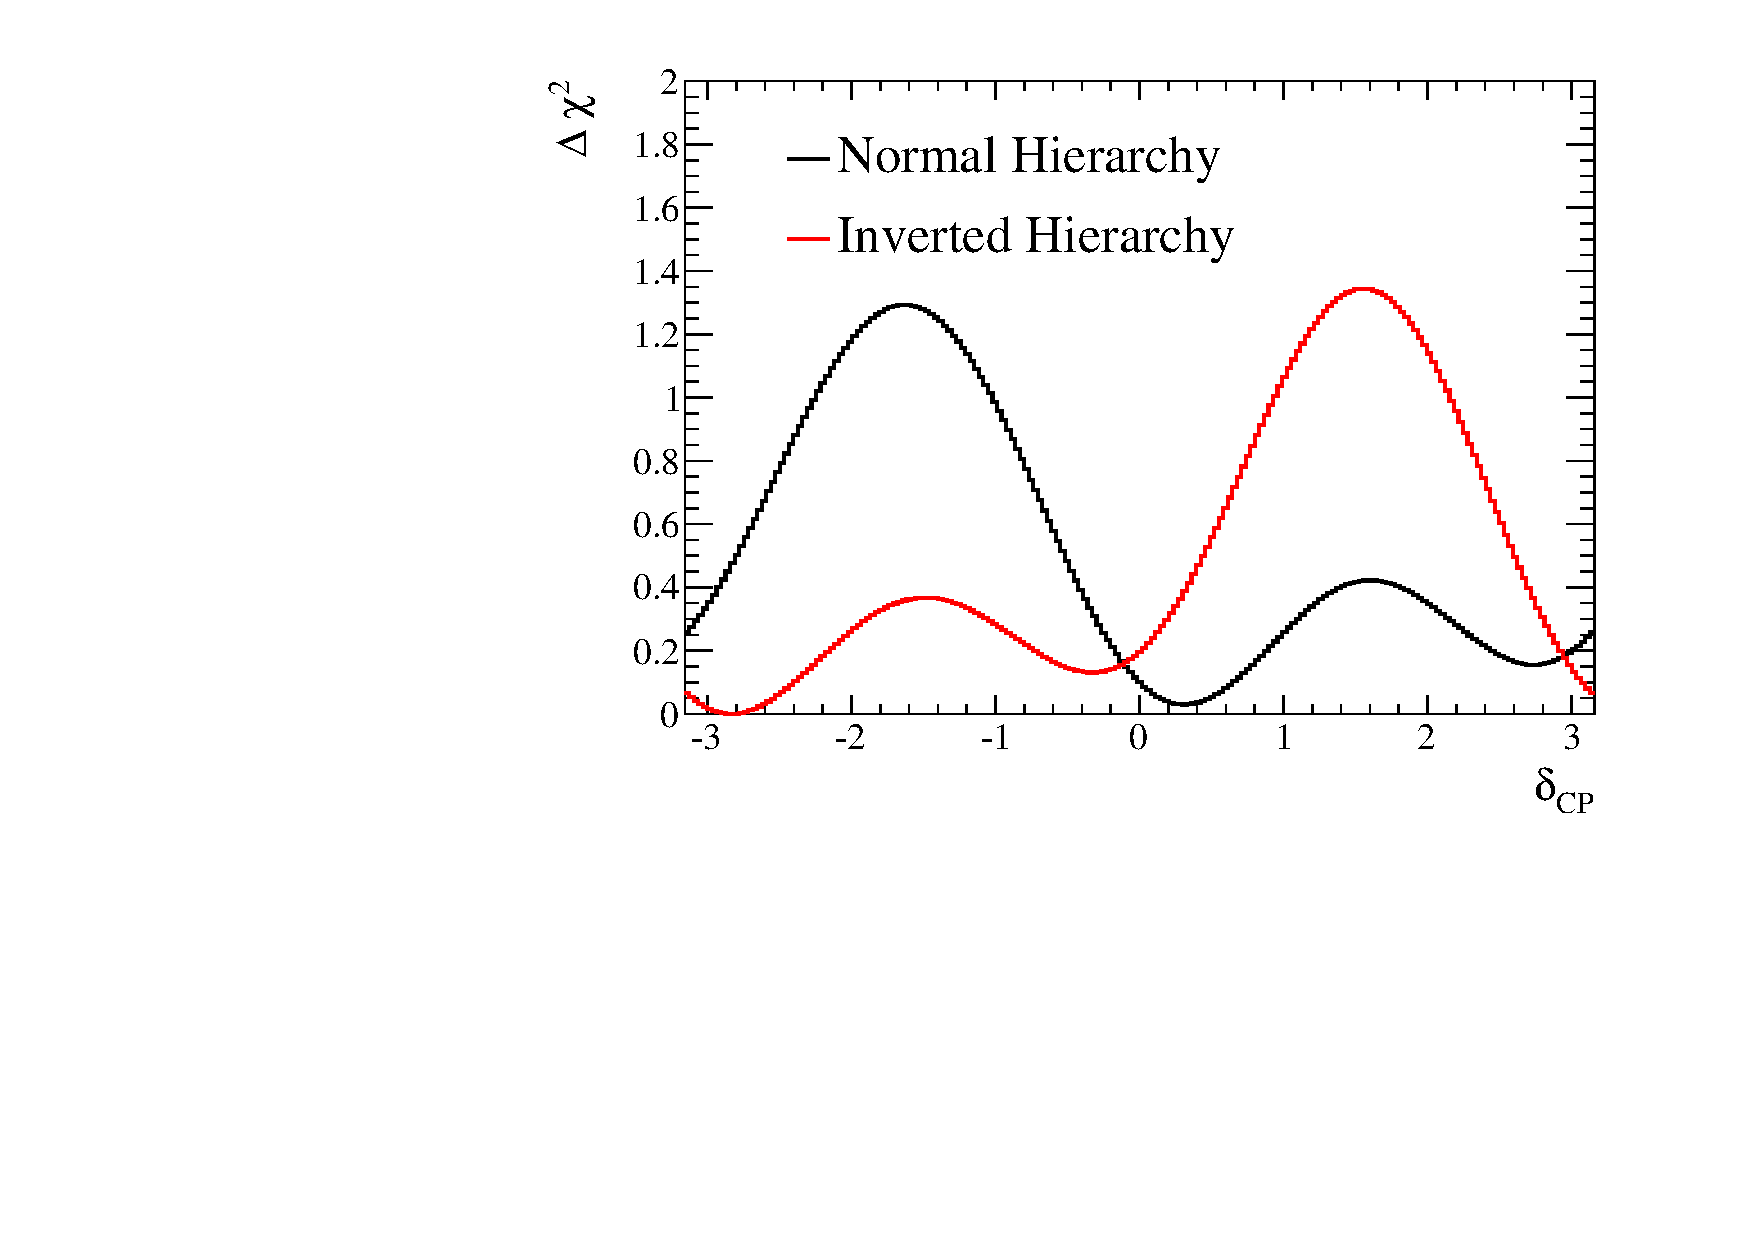
\includegraphics[width=0.9\textwidth]{./joint_plots/sensitivities/dcp_1D/dcp_react_Asimov_B.pdf} 
\caption{Asimov B: with reactor constraint}
\end{subfigure}
\begin{subfigure}[b]{0.49\textwidth}
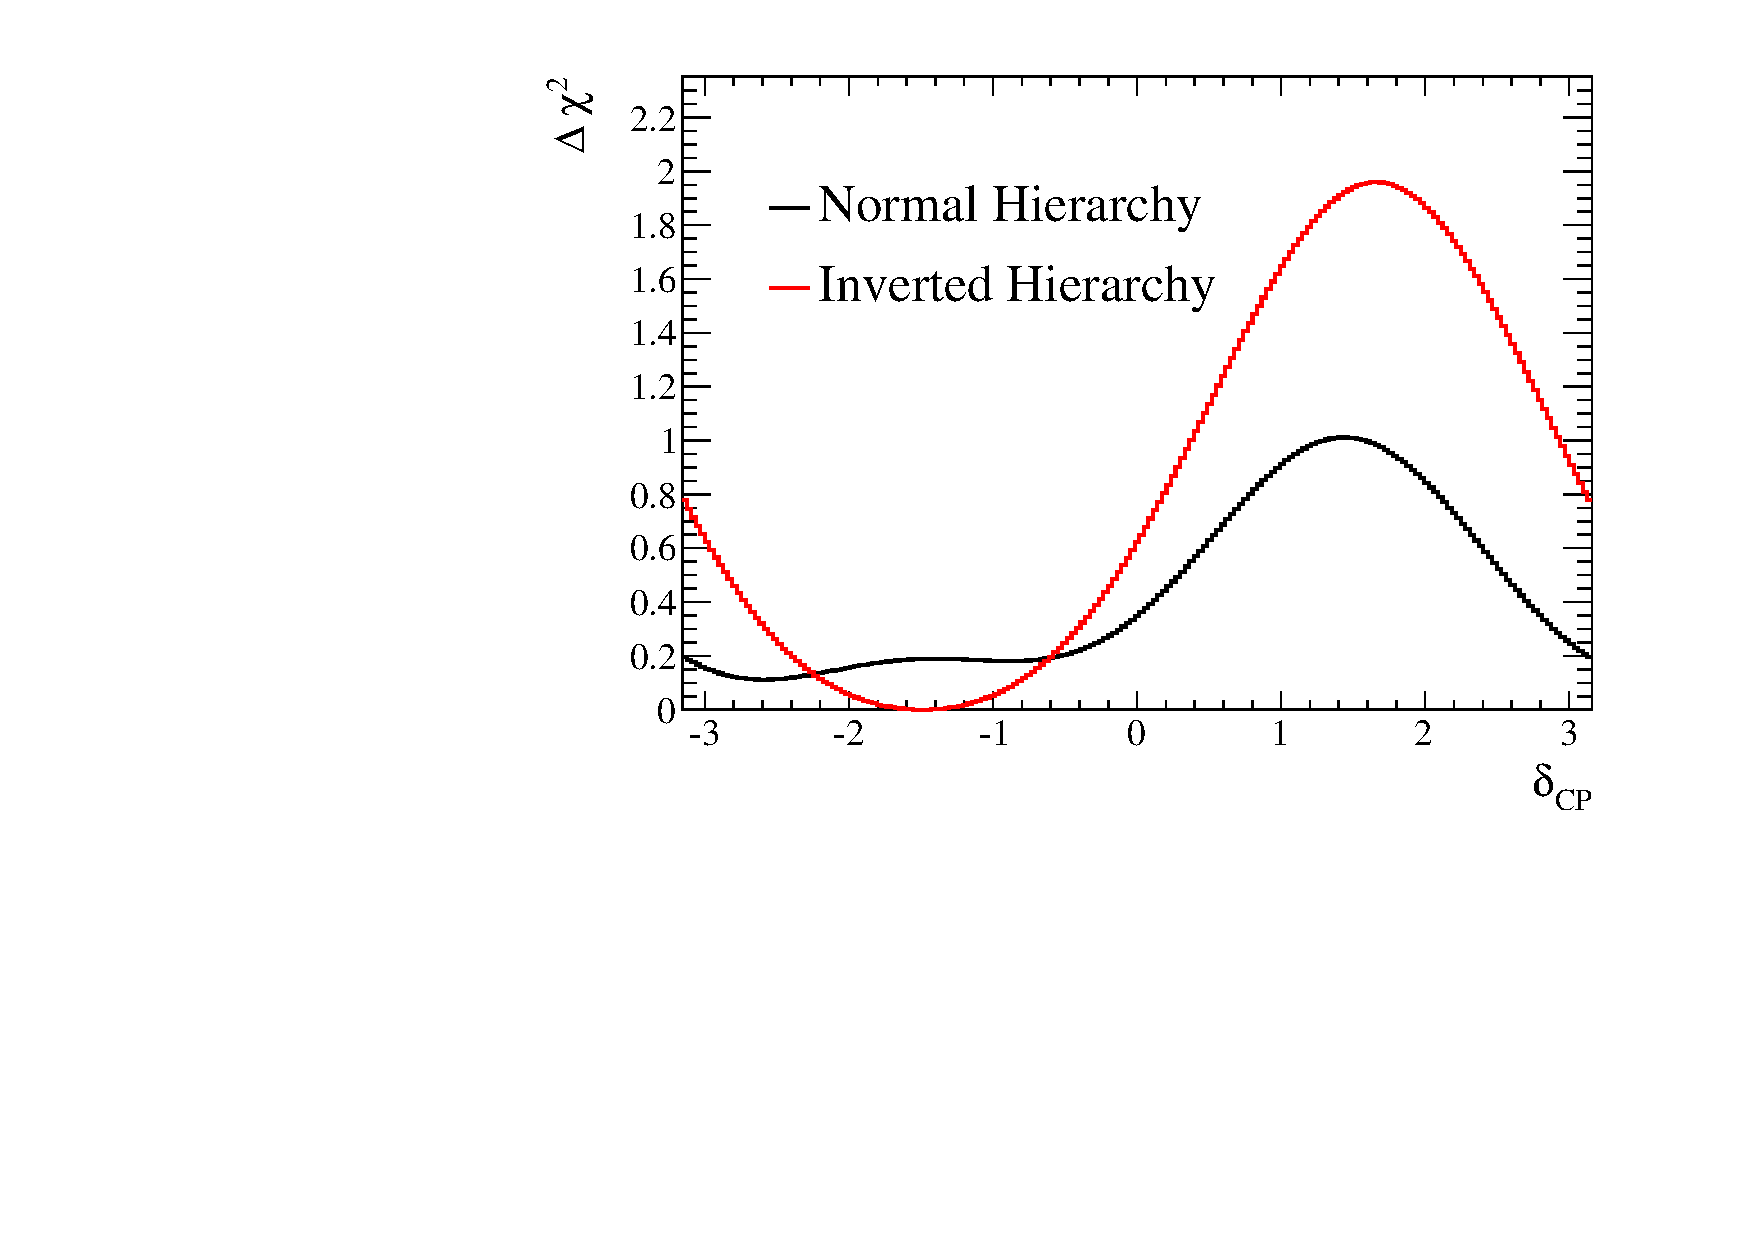
\includegraphics[width=0.9\textwidth]{./joint_plots/sensitivities/dcp_1D/dcp_t2konly_Asimov_A.pdf}
\caption{Asimov A: with T2K only}
\end{subfigure}
\begin{subfigure}[b]{0.49\textwidth}
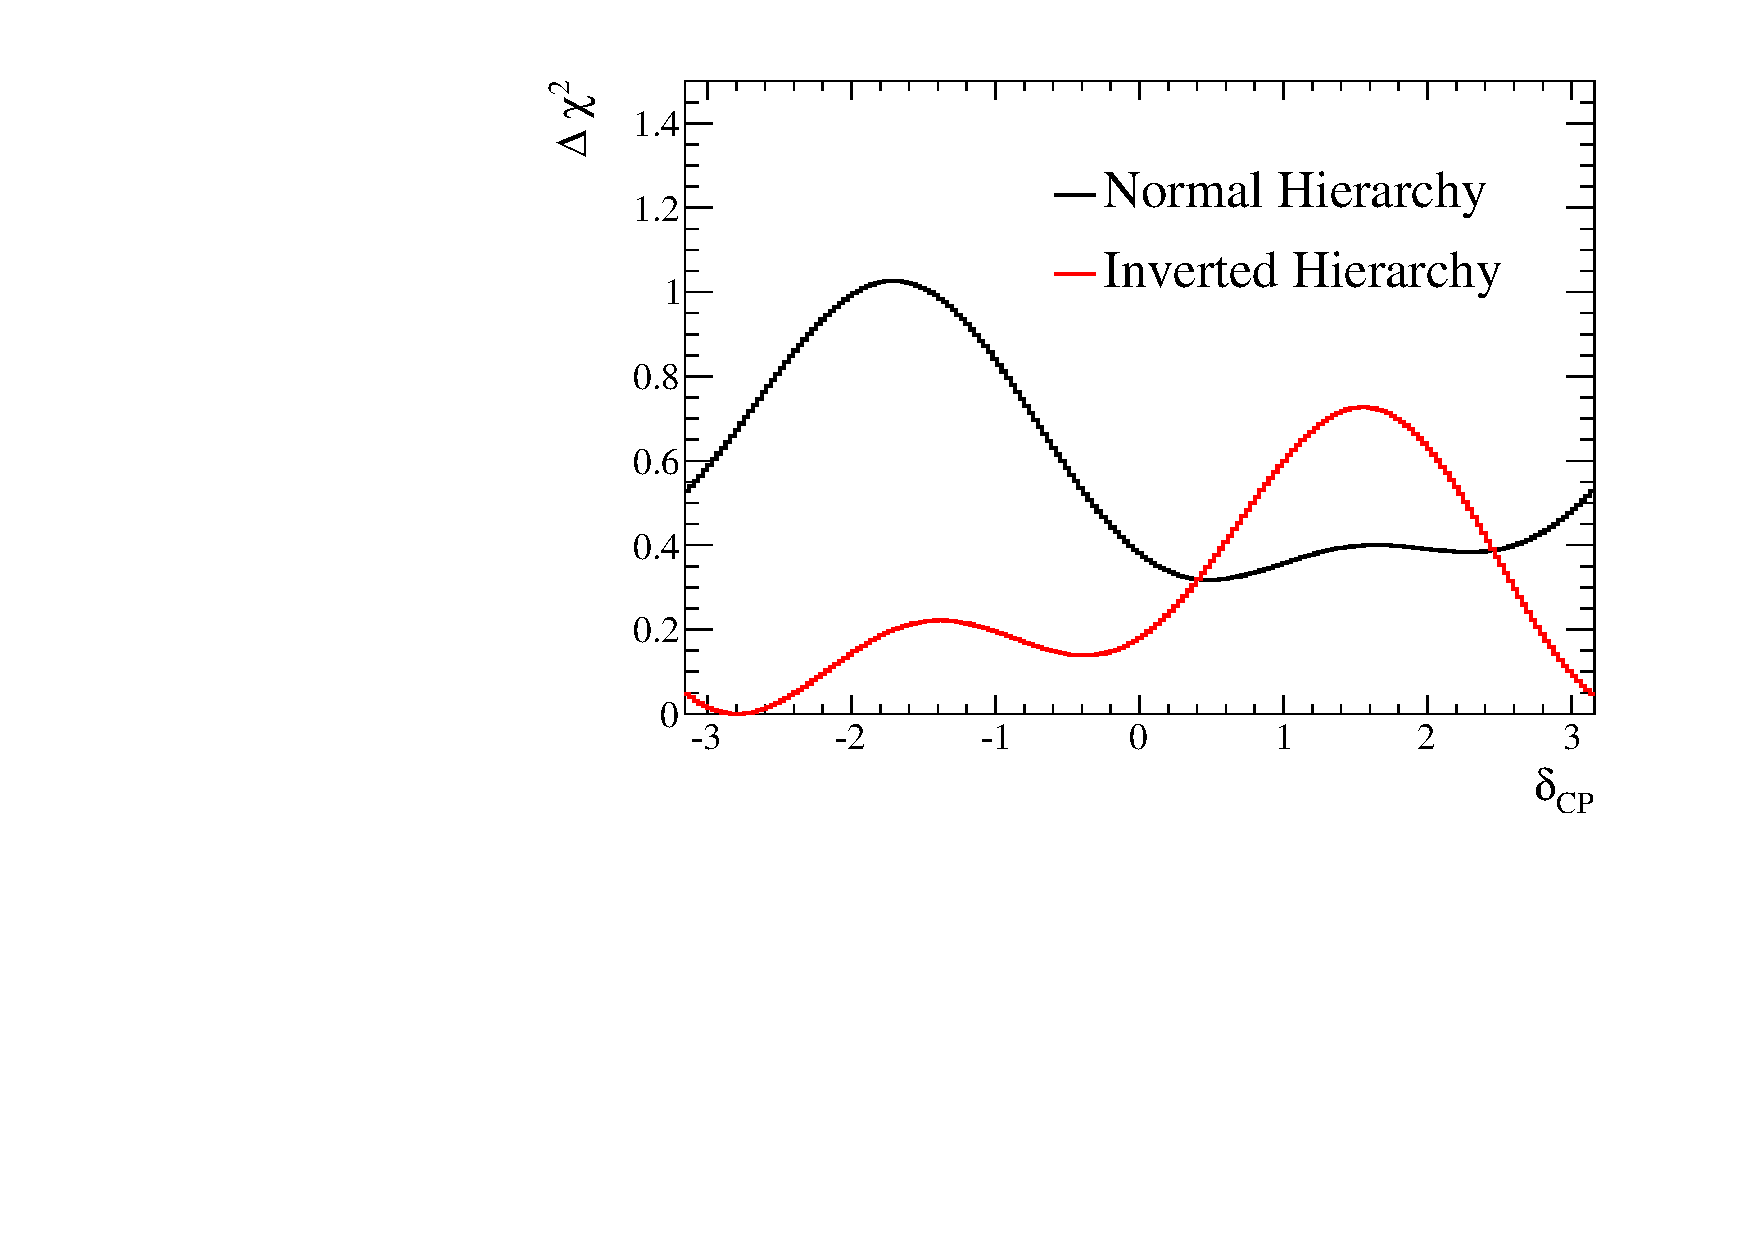
\includegraphics[width=0.9\textwidth]{./joint_plots/sensitivities/dcp_1D/dcp_t2konly_Asimov_B.pdf}
\caption{Asimov B: with T2K only}
\end{subfigure}
\caption {
%{\large{SENSI DELTACHISQ 1D DELTACP W/ AND W/O REACTORS}}
The expected $\Delta \chi^2$ distribution as a function of $\delta_{CP}$ 
for the Asimov data sets A and B of Tab.~\ref{tab:osc_params_joint_asimov} 
corresponding to the Run 1-6 statistics
is compared to the result obtained by the other analysis groups.
The mass hierarchy is minimized:
both the normal and inverted hierarchy $\chi^2$ distributions 
are shifted to the same global best-fit $\chi^2$ value,
which is taken as the minimum between normal and inverted hierarchy.
}
\label{fig:validation_sensi_dcp}
\end{figure*}

Also the sensitivity to $\sin^2 \theta_{13}$ Vs $\delta_{CP}$ 
with reactor constraint and T2K only data,
and $\sin^2 \theta_{23}$ Vs $m^2_{32}$ ($m^2_{13}$) with reactor constraint 
%compared to the ones of the other analyses groups,
are shown in Fig.~\ref{fig:validation_sensi_2d_reactors} 
and 
\ref{fig:validation_sensi_2d_t2konly},
where normal and inverted hierarchy contours are set independently,
i.e. each calculated with respect to its own minimum $\chi^2$ value
and not the global minimum as a function of the mass hierarchy.

\begin{figure*}[htb]
\center
%
\includegraphics[width=0.9\textwidth]{./images/missing_plot-eps-converted-to.pdf}
%
\includegraphics[width=0.9\textwidth]{./images/missing_plot-eps-converted-to.pdf}
%
\includegraphics[width=0.9\textwidth]{./images/missing_plot-eps-converted-to.pdf}
%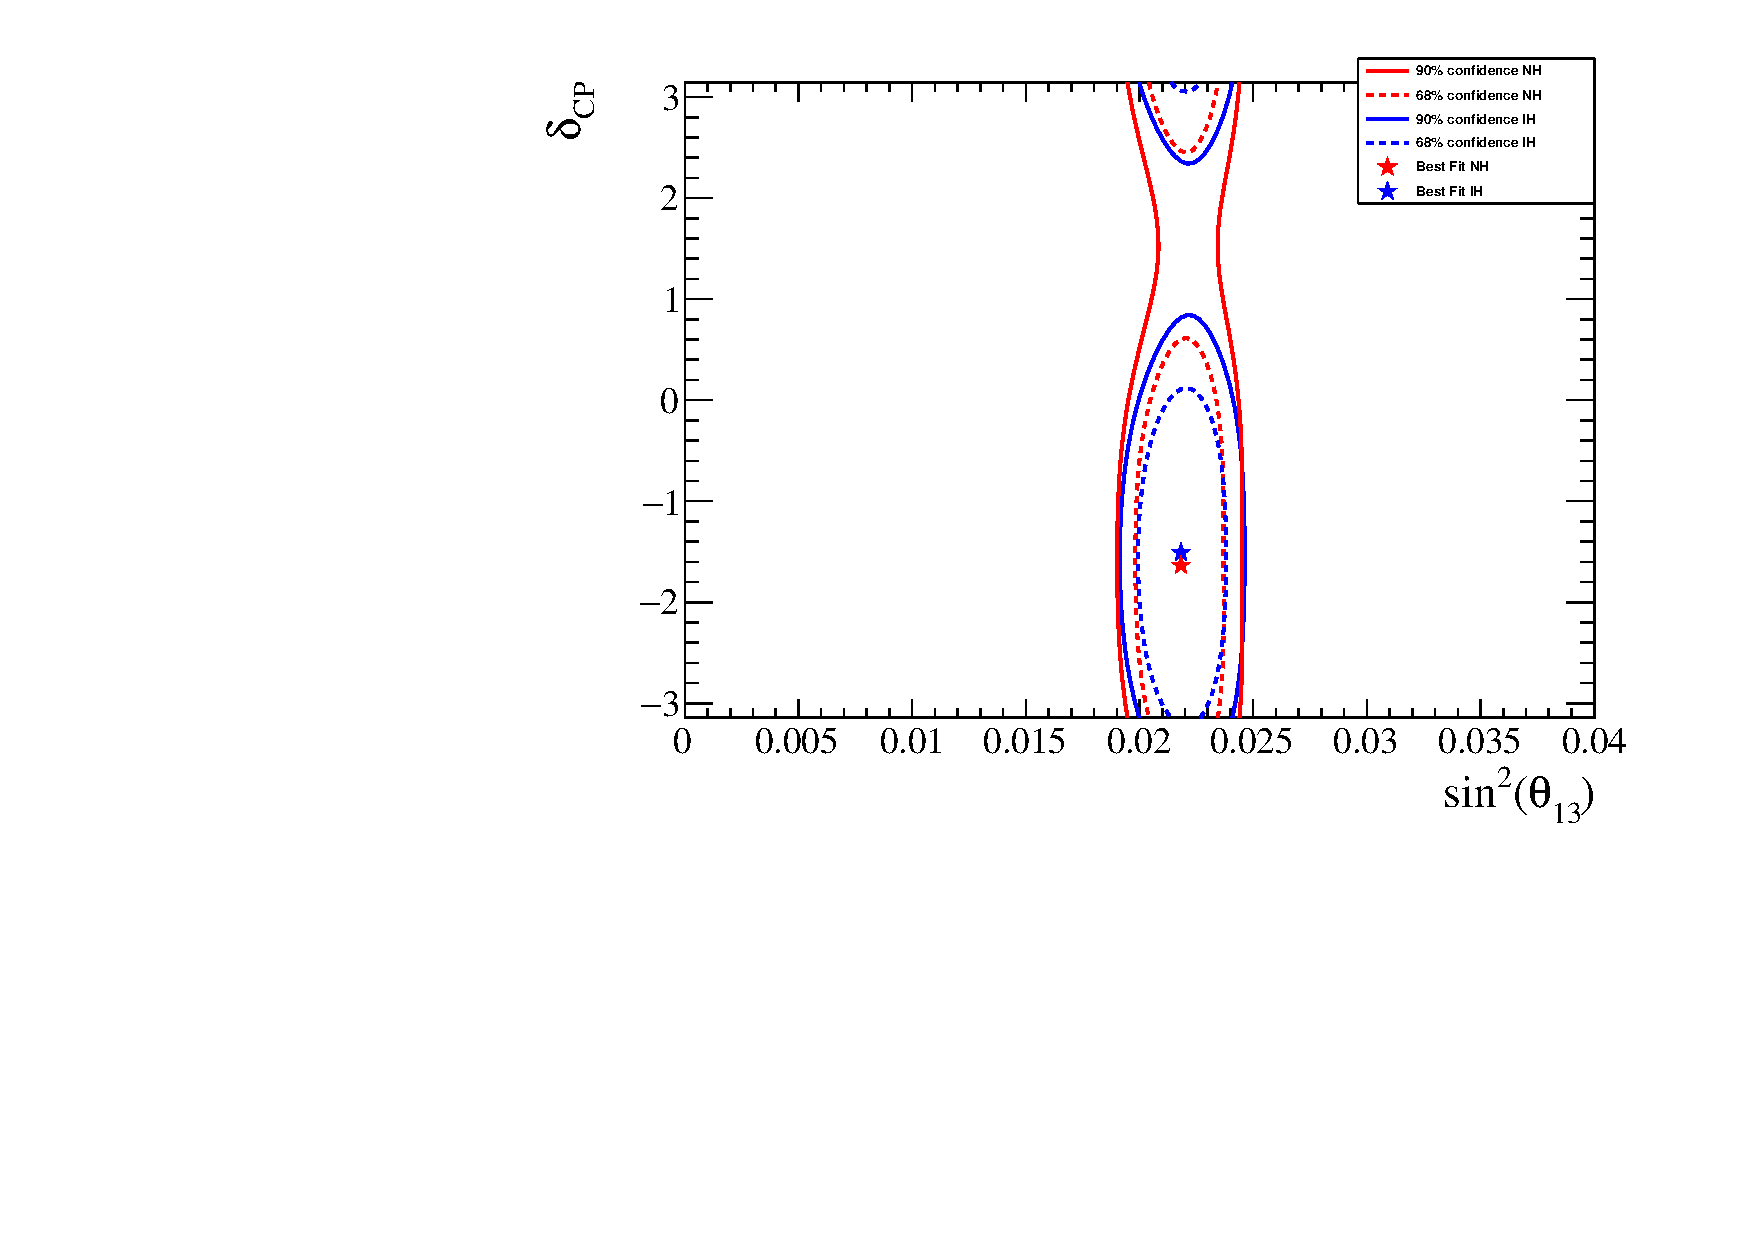
\includegraphics[width=0.9\textwidth]{./joint_plots/sensitivities/2D/cp13_reactor/cp13_reactor_A.pdf}
%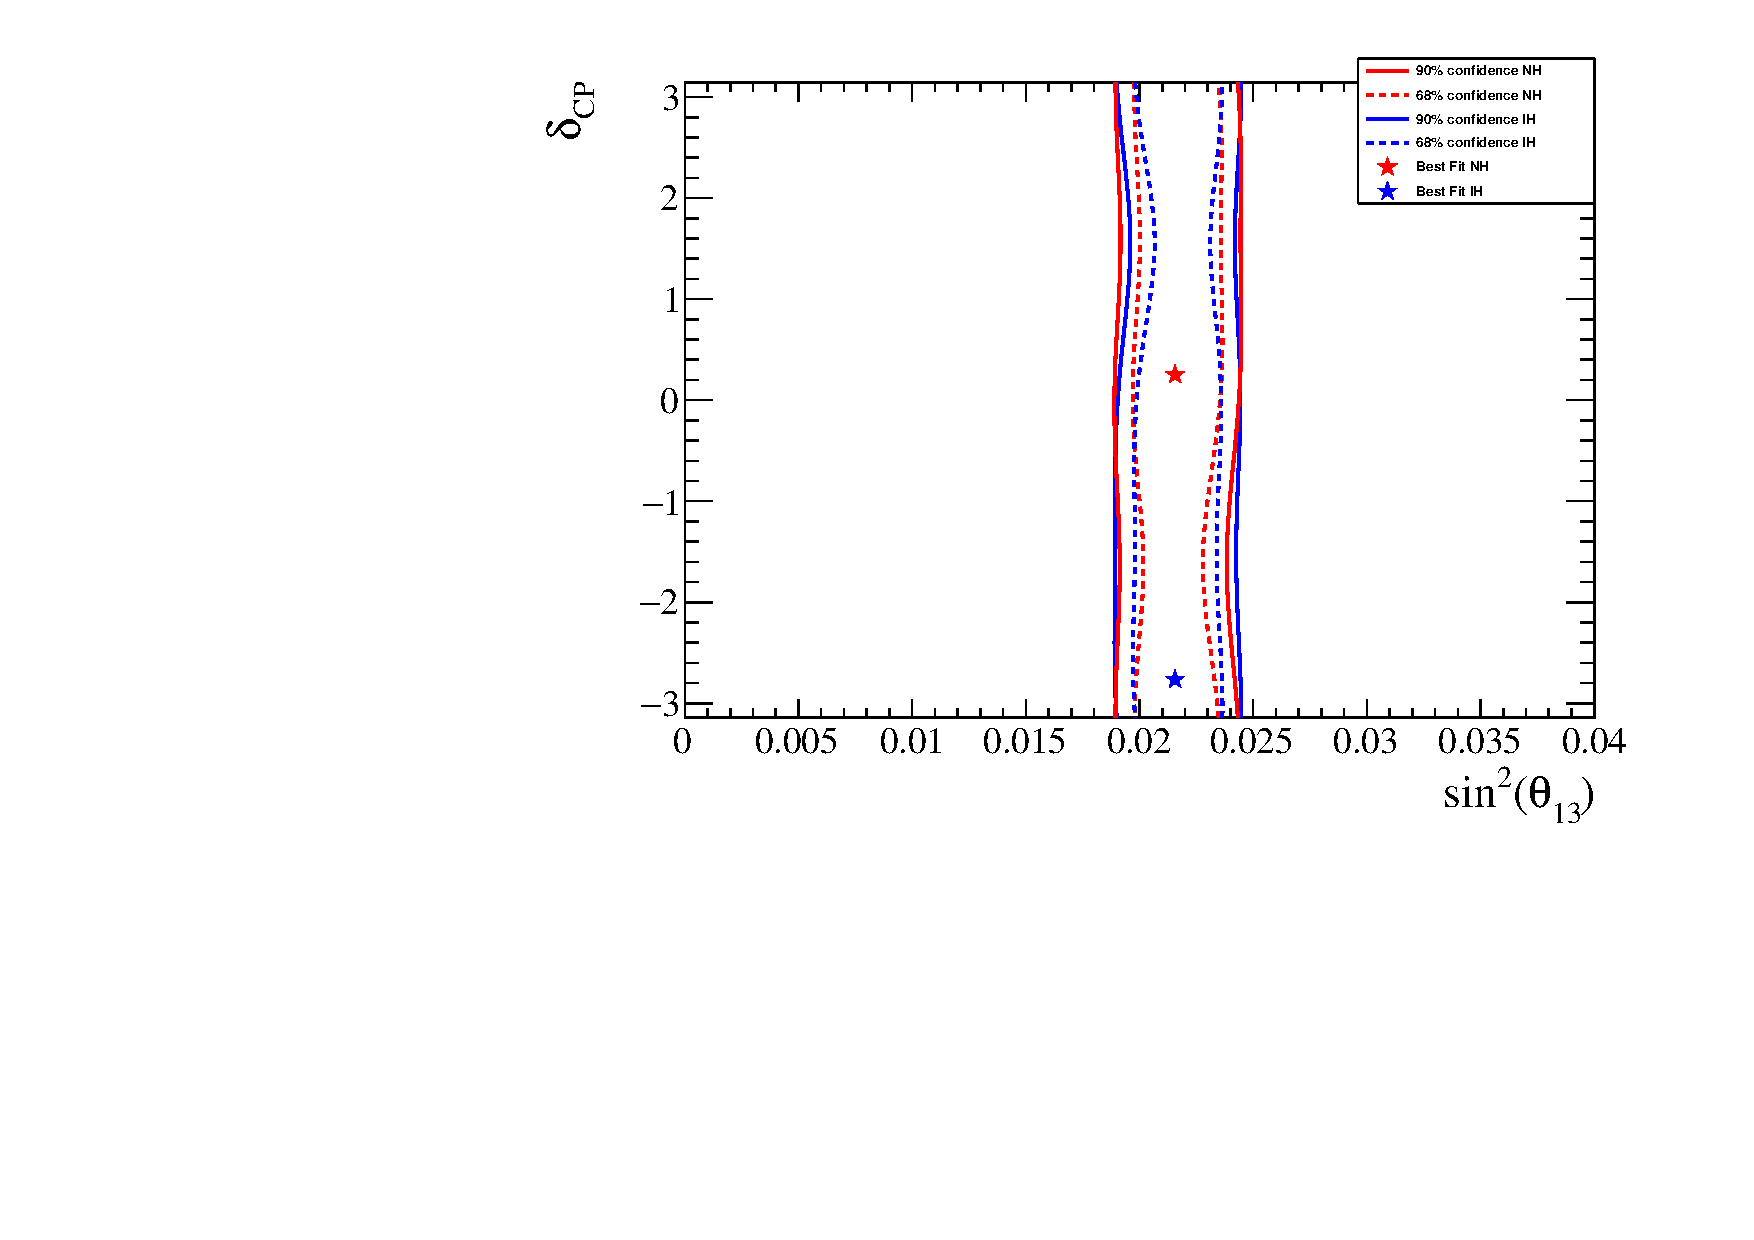
\includegraphics[width=0.9\textwidth]{./joint_plots/sensitivities/2D/cp13_reactor/cp13_reactor_B.pdf}
%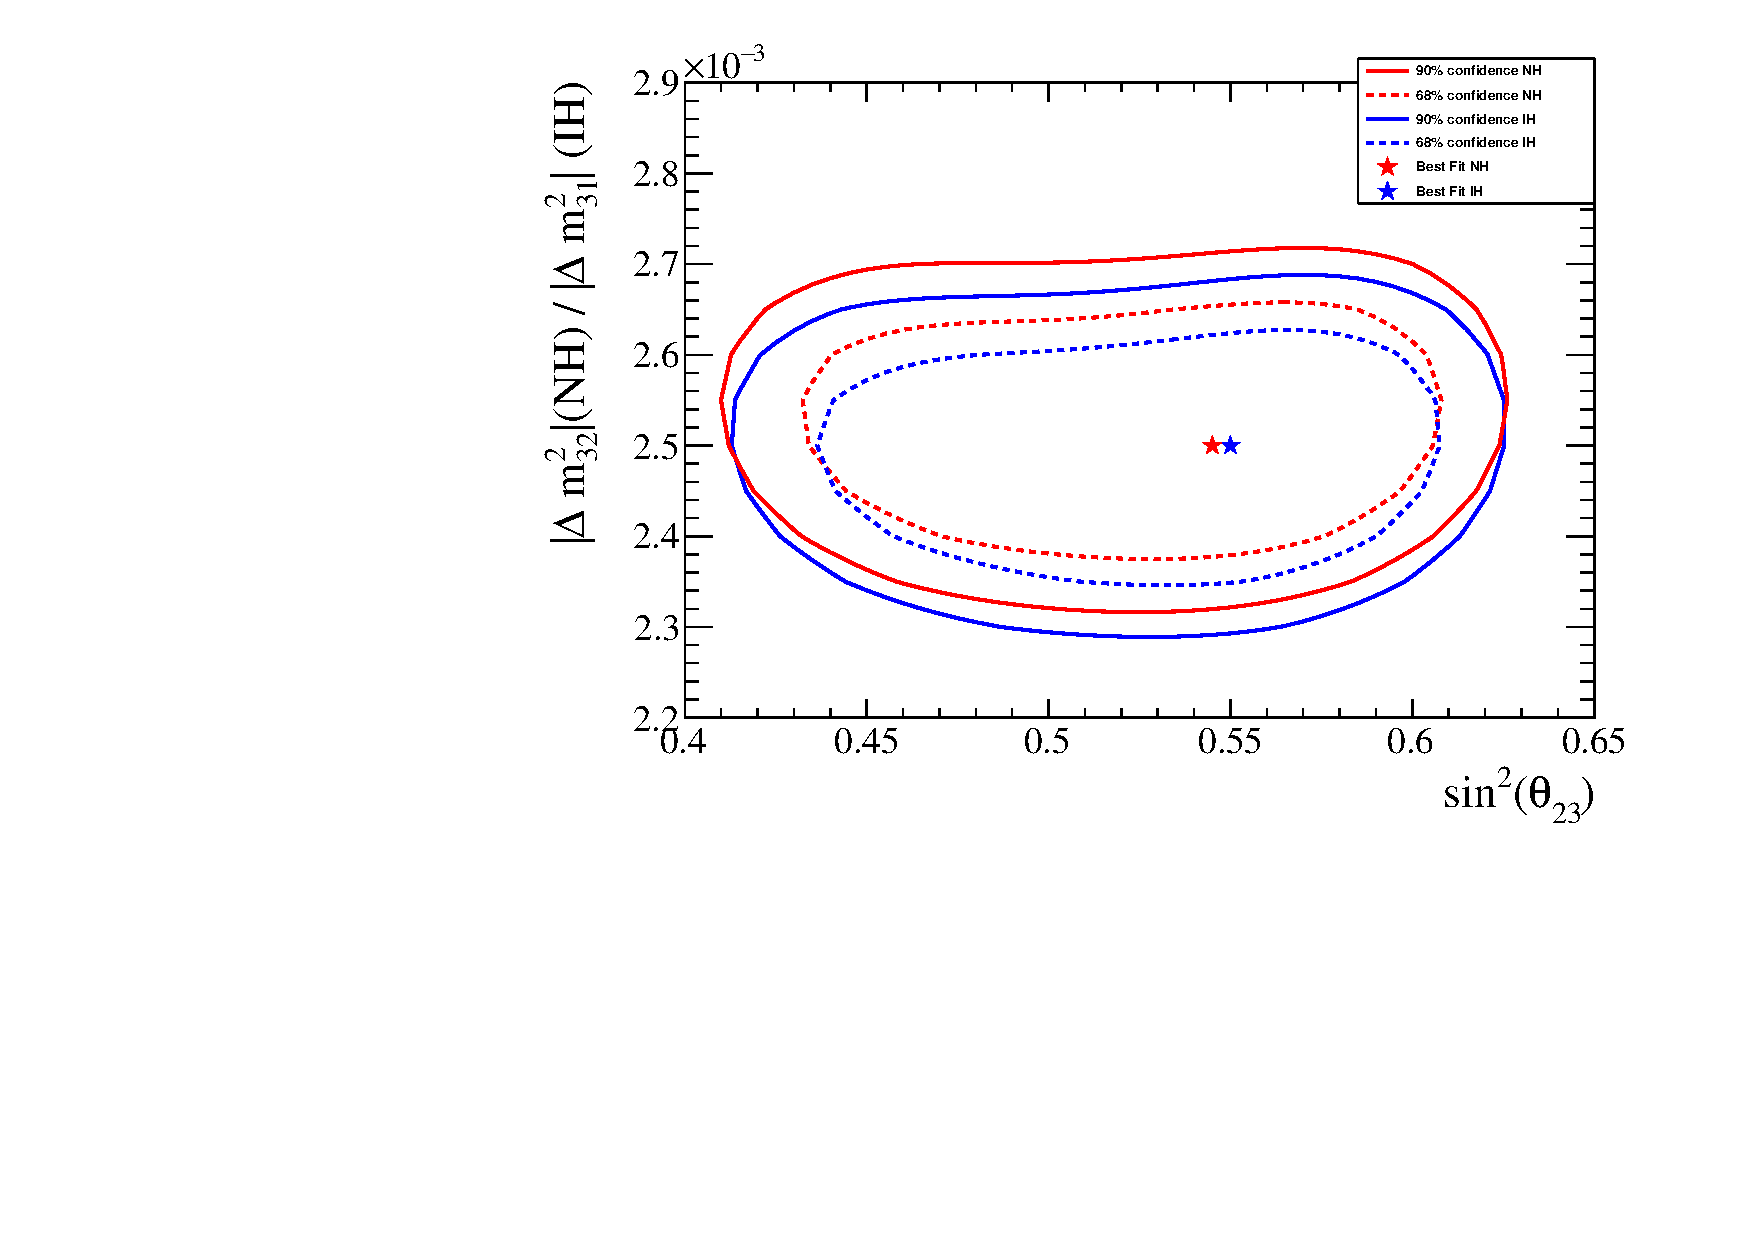
\includegraphics[width=0.9\textwidth]{./joint_plots/sensitivities/2D/ss23dmsq/ss23dmsq_A.pdf}
%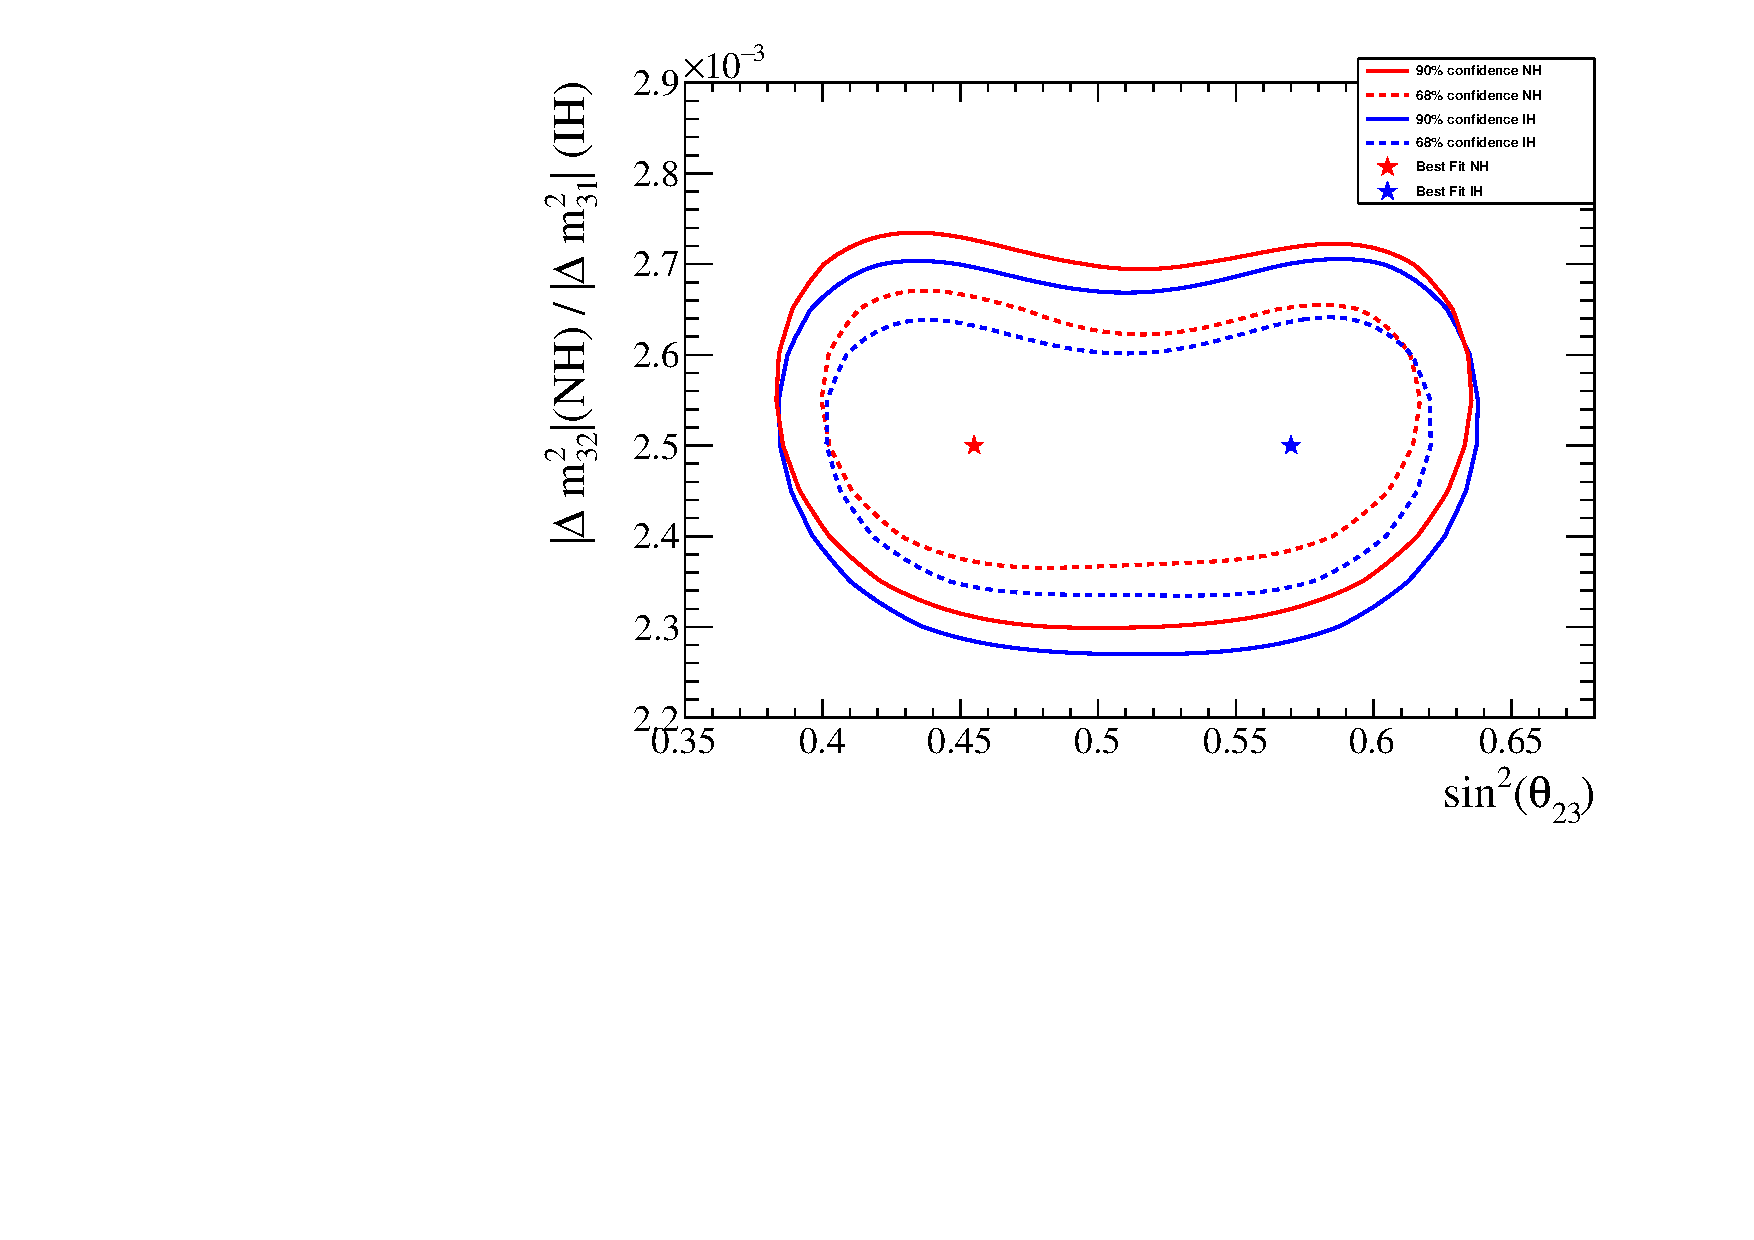
\includegraphics[width=0.9\textwidth]{./joint_plots/sensitivities/2D/ss23dmsq/ss23dmsq_B.pdf}
\begin{subfigure}[b]{0.49\textwidth}
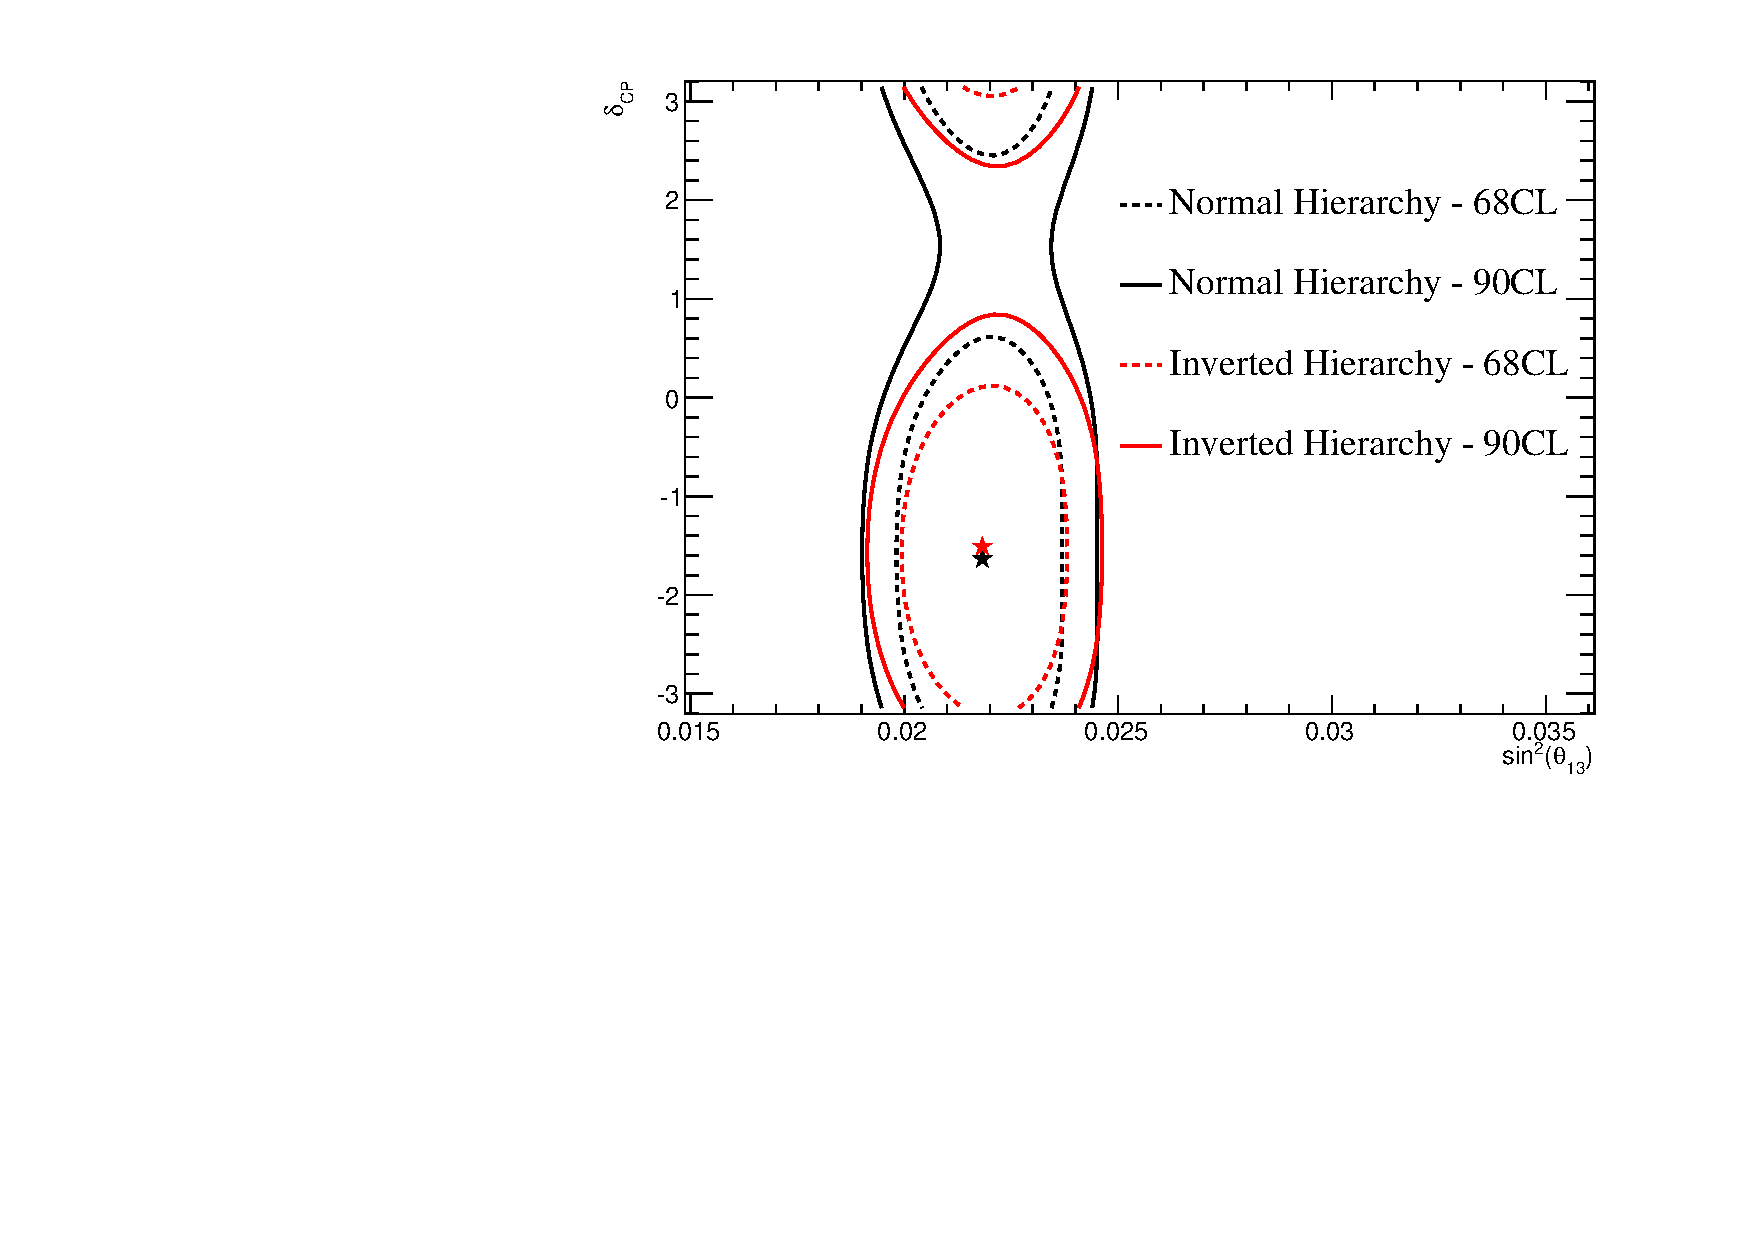
\includegraphics[width=0.9\textwidth]{./joint_plots/sensitivities/2D/contour_joint_sinsqth13Vsdcp_Asimov_A_react}
\caption{Asimov A: $\sin^2 \theta_{13}$ Vs $\delta_{CP}$}
\end{subfigure}
\begin{subfigure}[b]{0.49\textwidth}
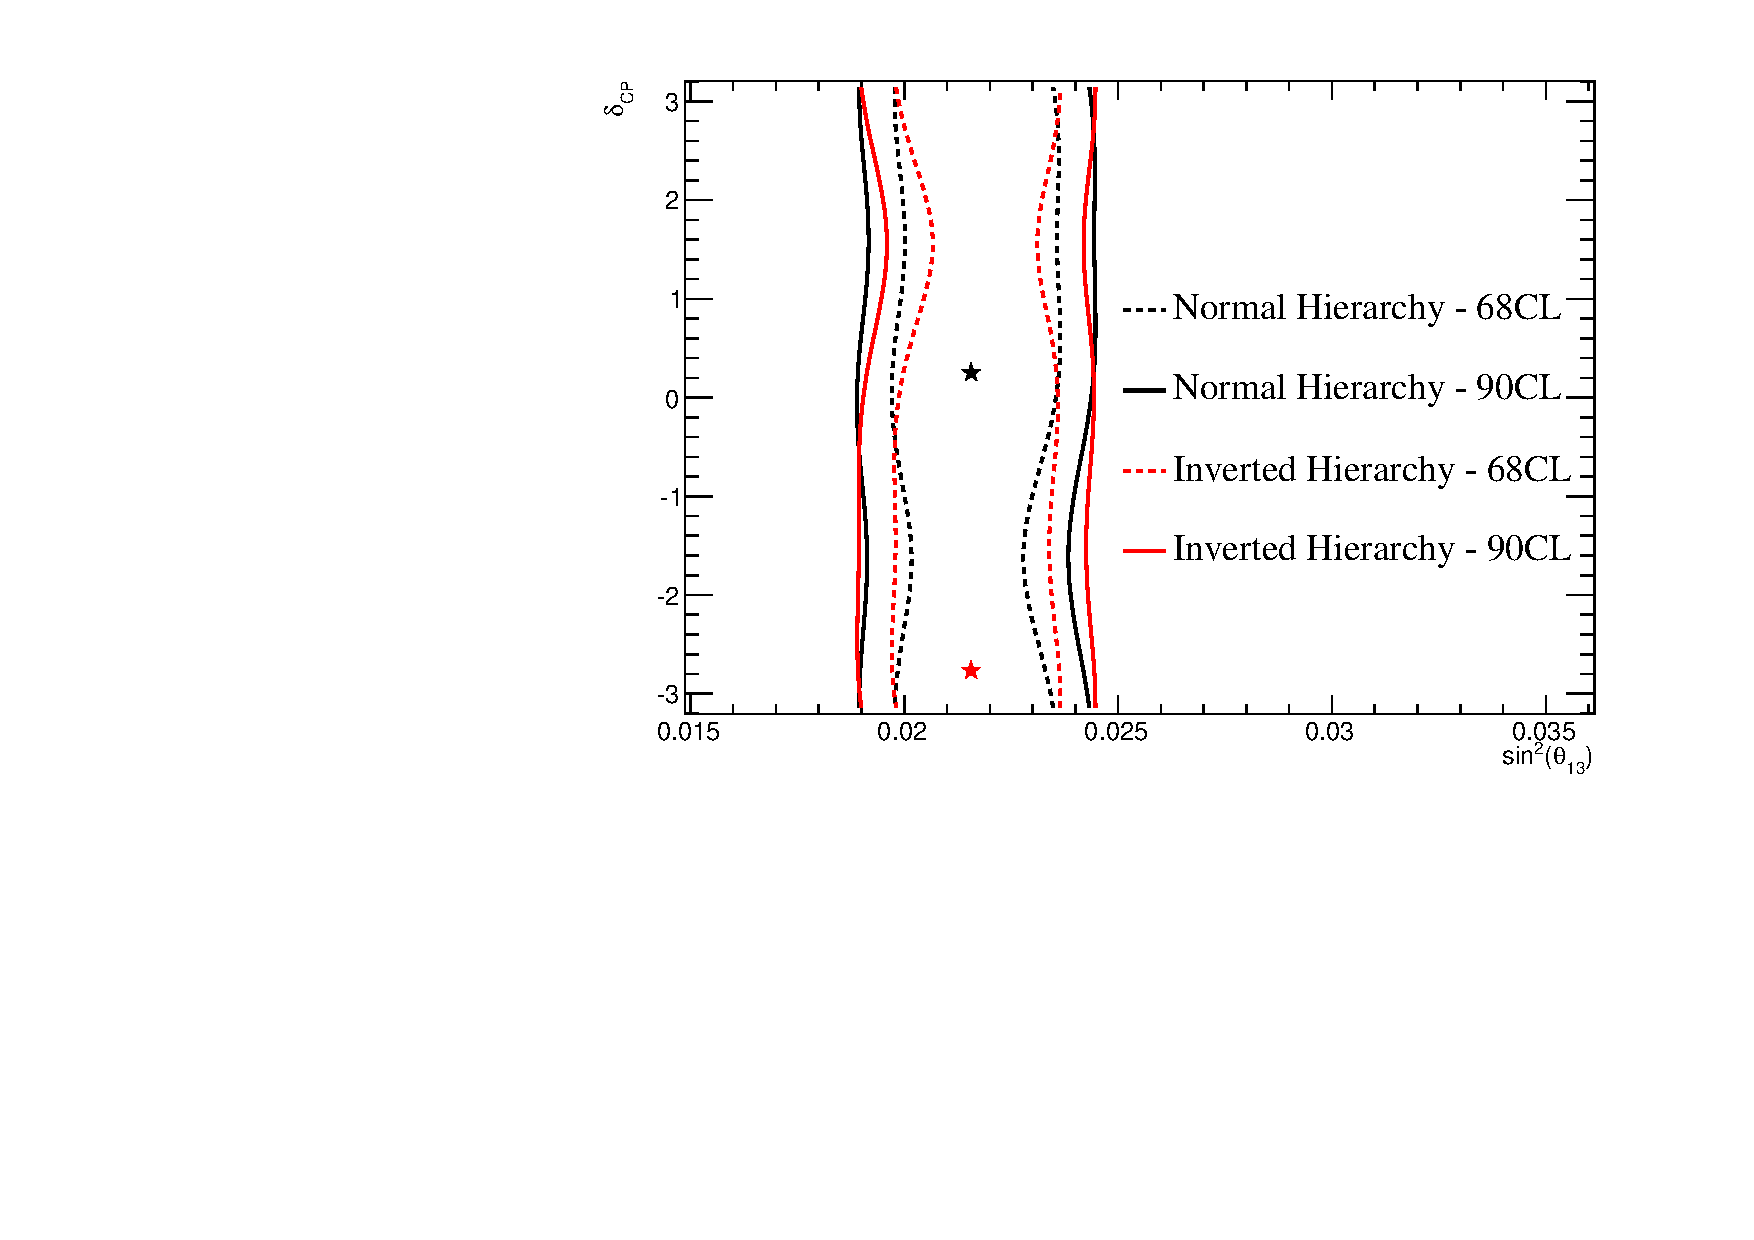
\includegraphics[width=0.9\textwidth]{./joint_plots/sensitivities/2D/contour_joint_sinsqth13Vsdcp_Asimov_B_react} 
\caption{Asimov B: $\sin^2 \theta_{13}$ Vs $\delta_{CP}$}
\end{subfigure}
\begin{subfigure}[b]{0.49\textwidth}
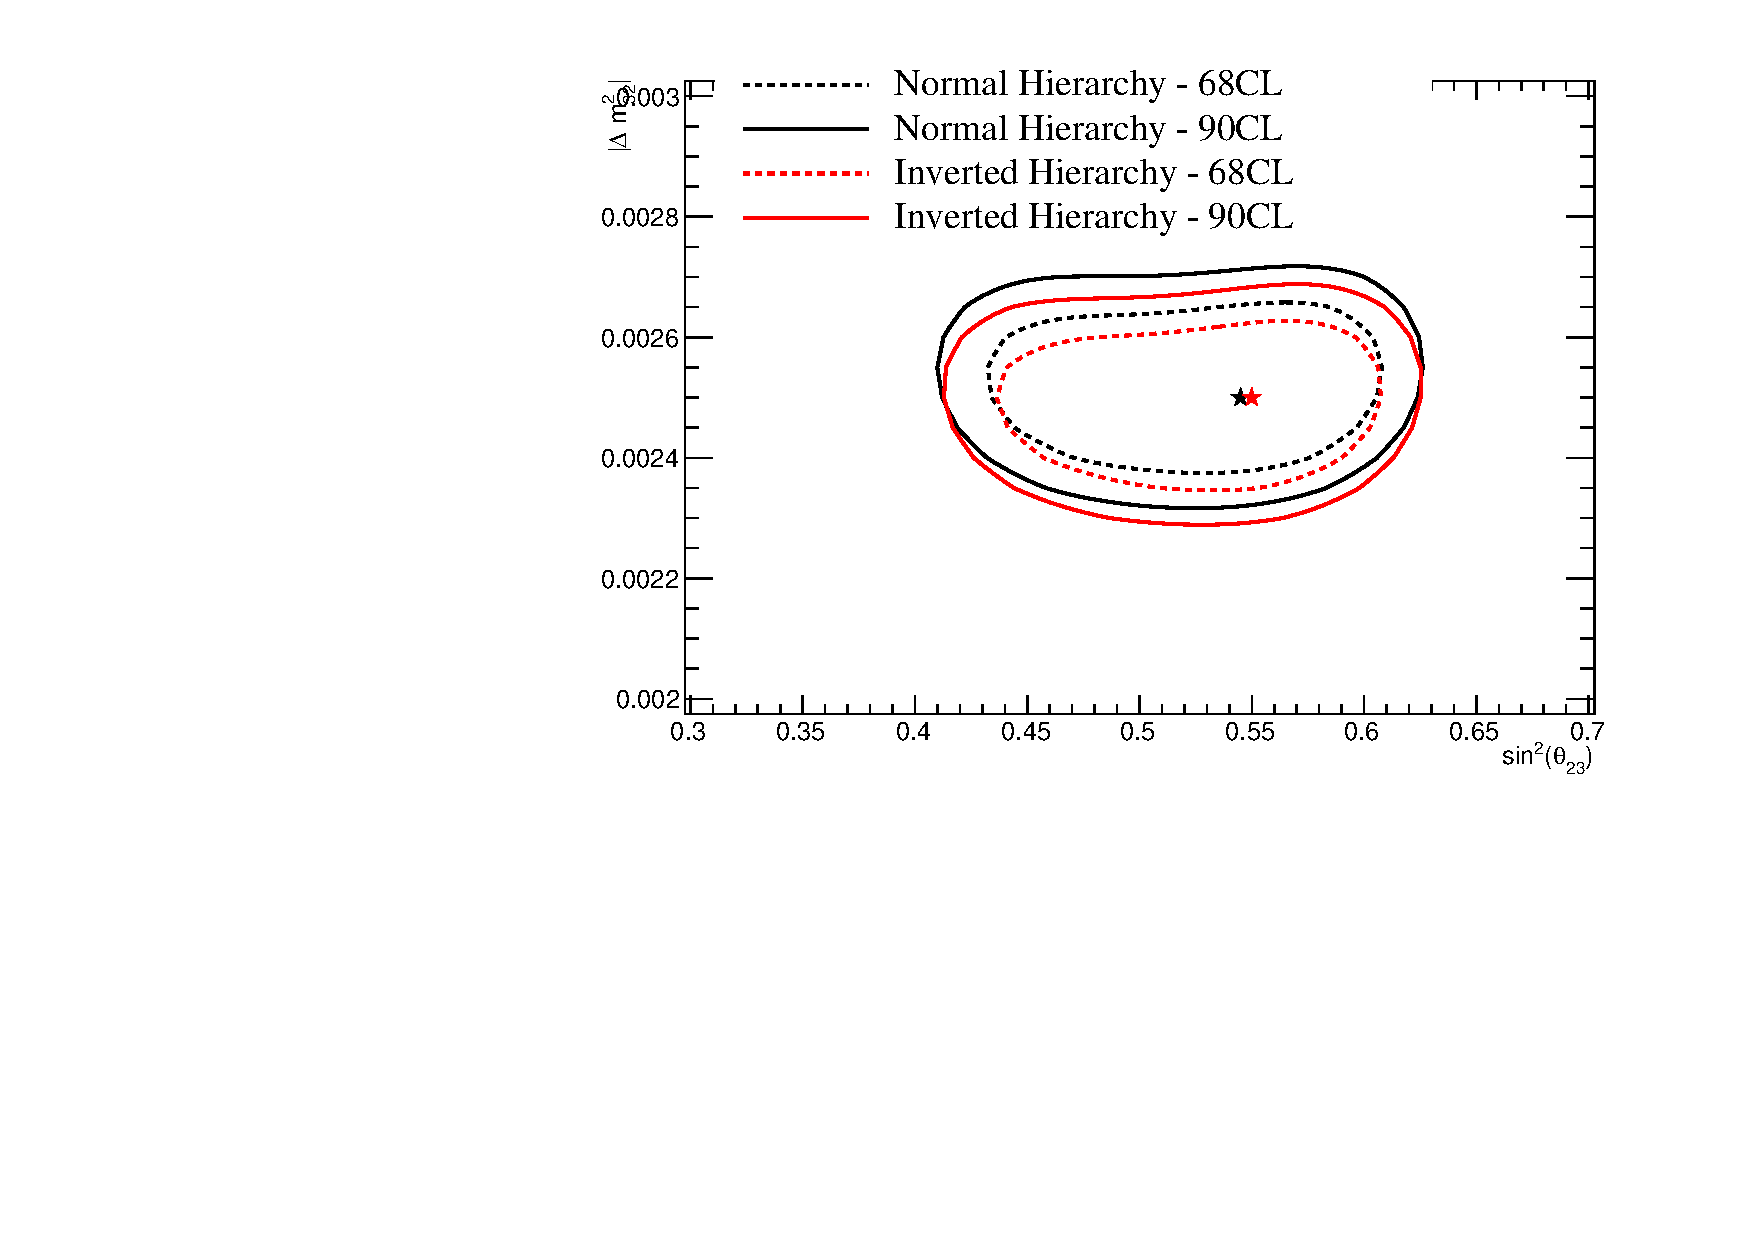
\includegraphics[width=0.9\textwidth]{./joint_plots/sensitivities/2D/contour_joint_sinsqth23Vsdmsq_Asimov_A_react}
\caption{Asimov A: $\sin^2 \theta_{23}$ Vs $\Delta m^2_{32}$ ($m^2_{13}$)}
\end{subfigure}
\begin{subfigure}[b]{0.49\textwidth}
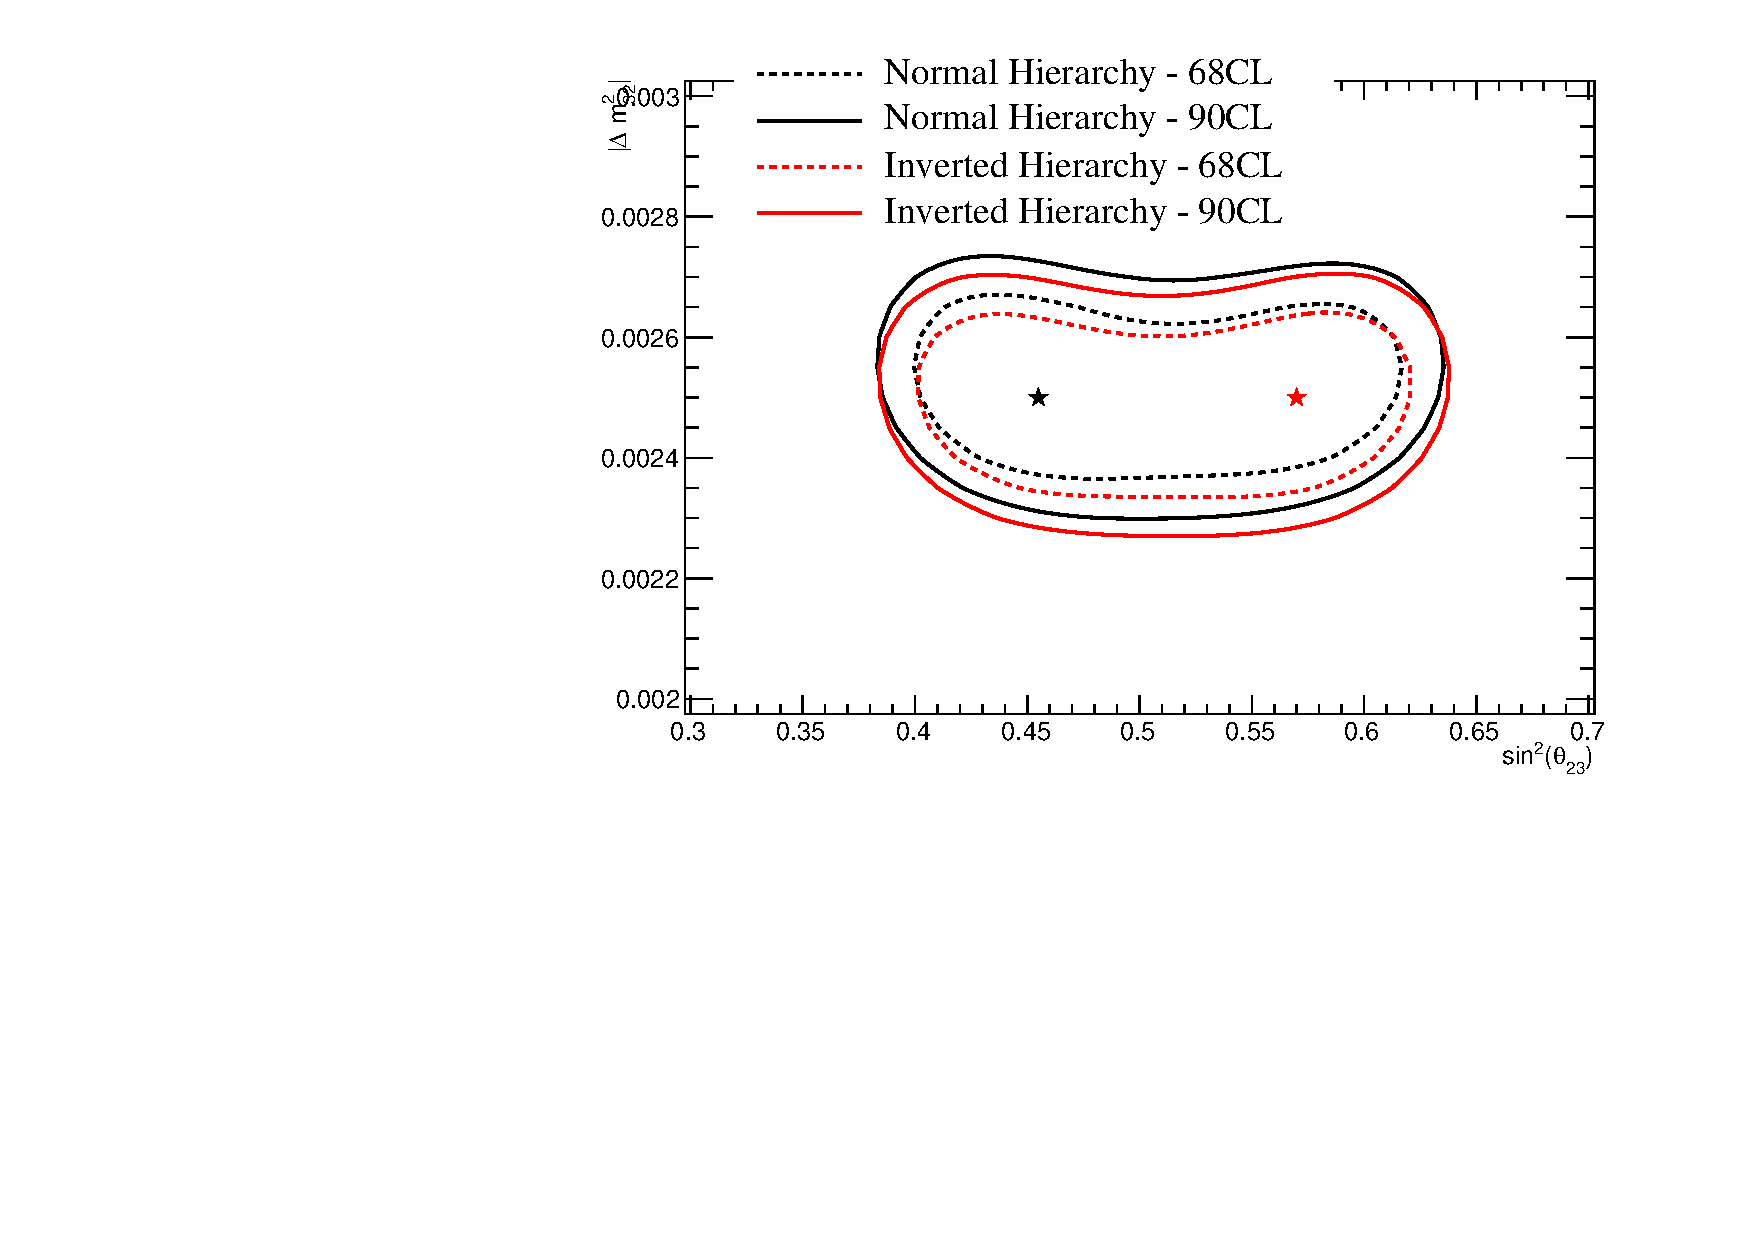
\includegraphics[width=0.9\textwidth]{./joint_plots/sensitivities/2D/contour_joint_sinsqth23Vsdmsq_Asimov_B_react}
\caption{Asimov B: $\sin^2 \theta_{23}$ Vs $\Delta m^2_{32}$ ($m^2_{13}$)}
\end{subfigure}
\caption {
%{\large{SENSI 2D CONTOURS W/ AND W/O REACTORS}}
The contours at 68\% and 90\% CL with reactor constraint 
for the Asimov data sets A and B of tab.~\ref{tab:osc_params_joint_asimov} 
corresponding to the Run 1-6 statistics 
is shown.
%is compared to the result obtained by the other analysis groups.
Normal and inverted hierarchy contours are independent.
}
\label{fig:validation_sensi_2d_reactors}
\end{figure*}

\begin{figure*}[htb]
\center
\begin{subfigure}[b]{0.49\textwidth}
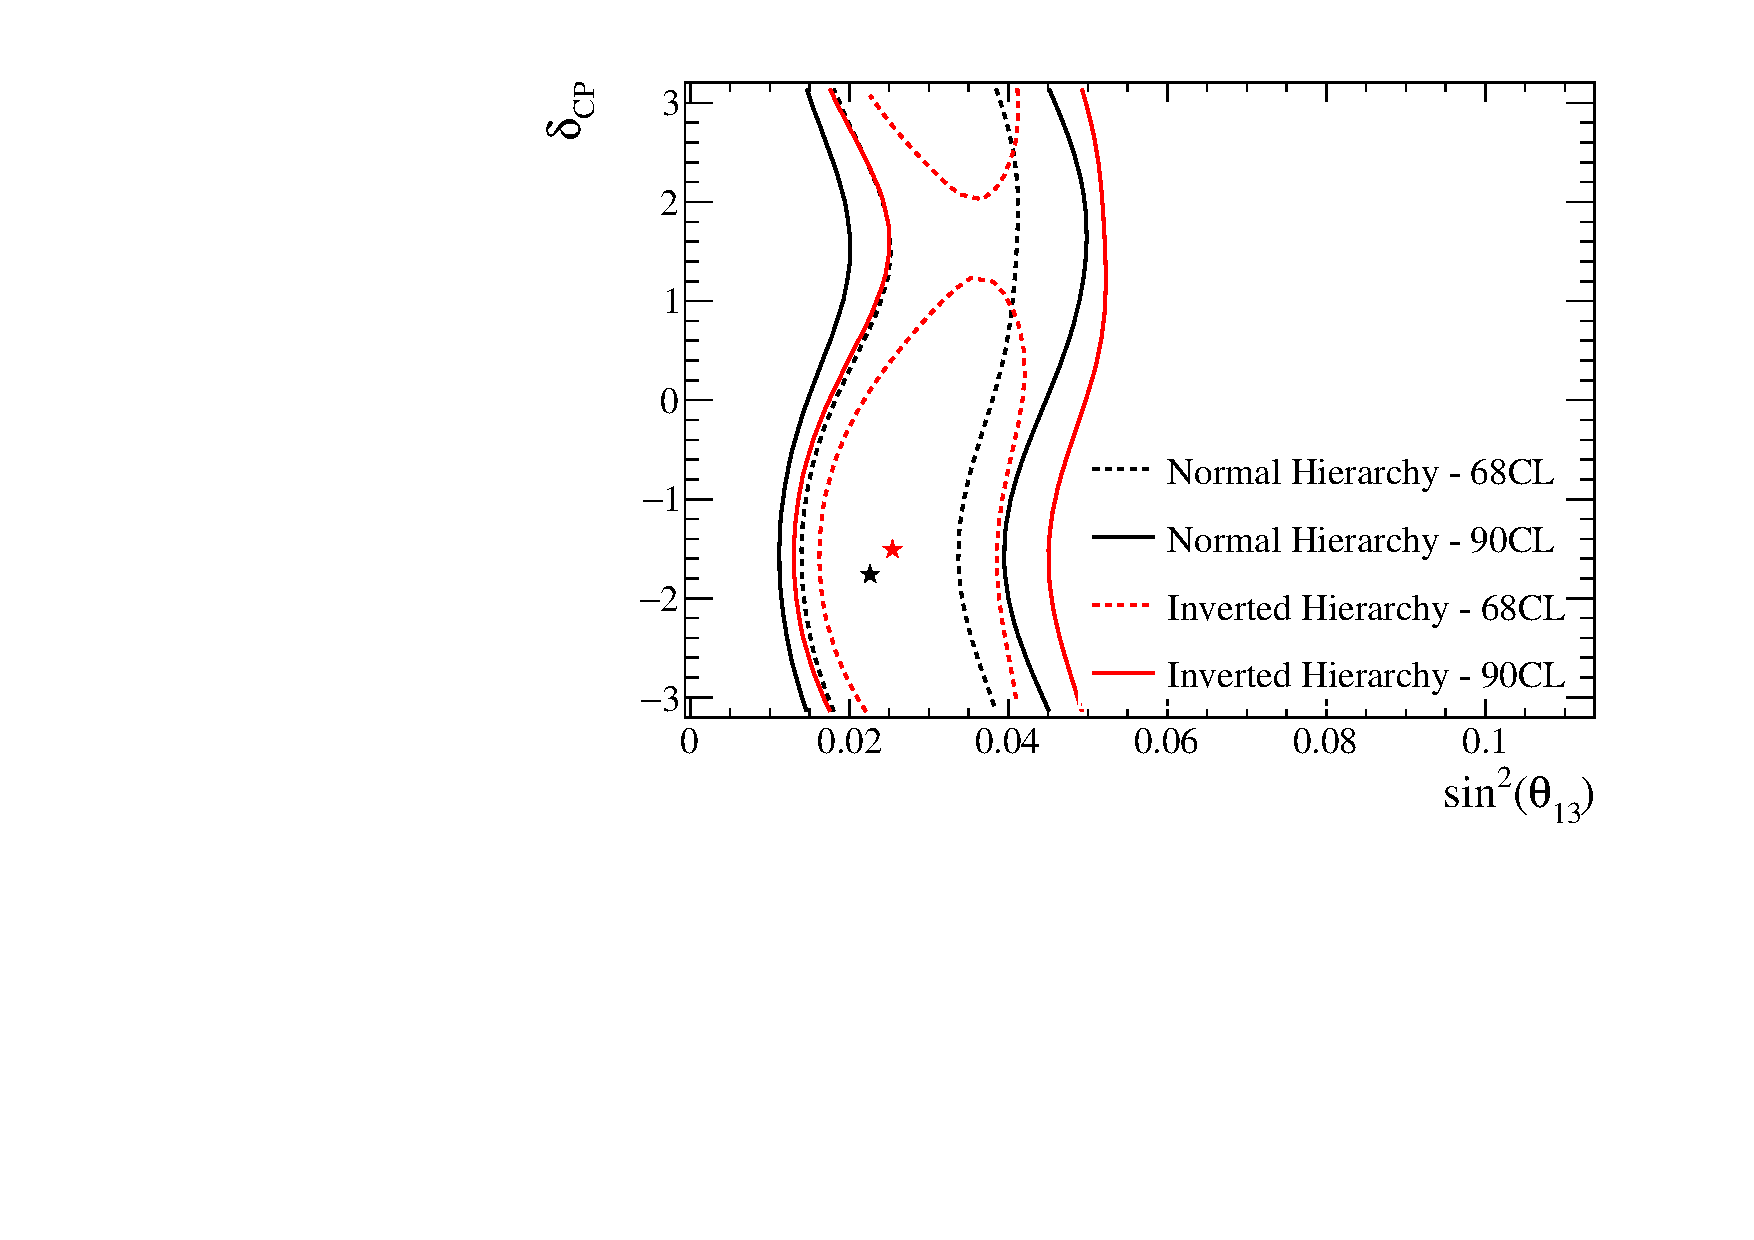
\includegraphics[width=0.9\textwidth]{./joint_plots/sensitivities/2D/cp13/cp13_A.pdf}
\caption{Asimov A with reactor constraint}
\end{subfigure}
\begin{subfigure}[b]{0.49\textwidth}
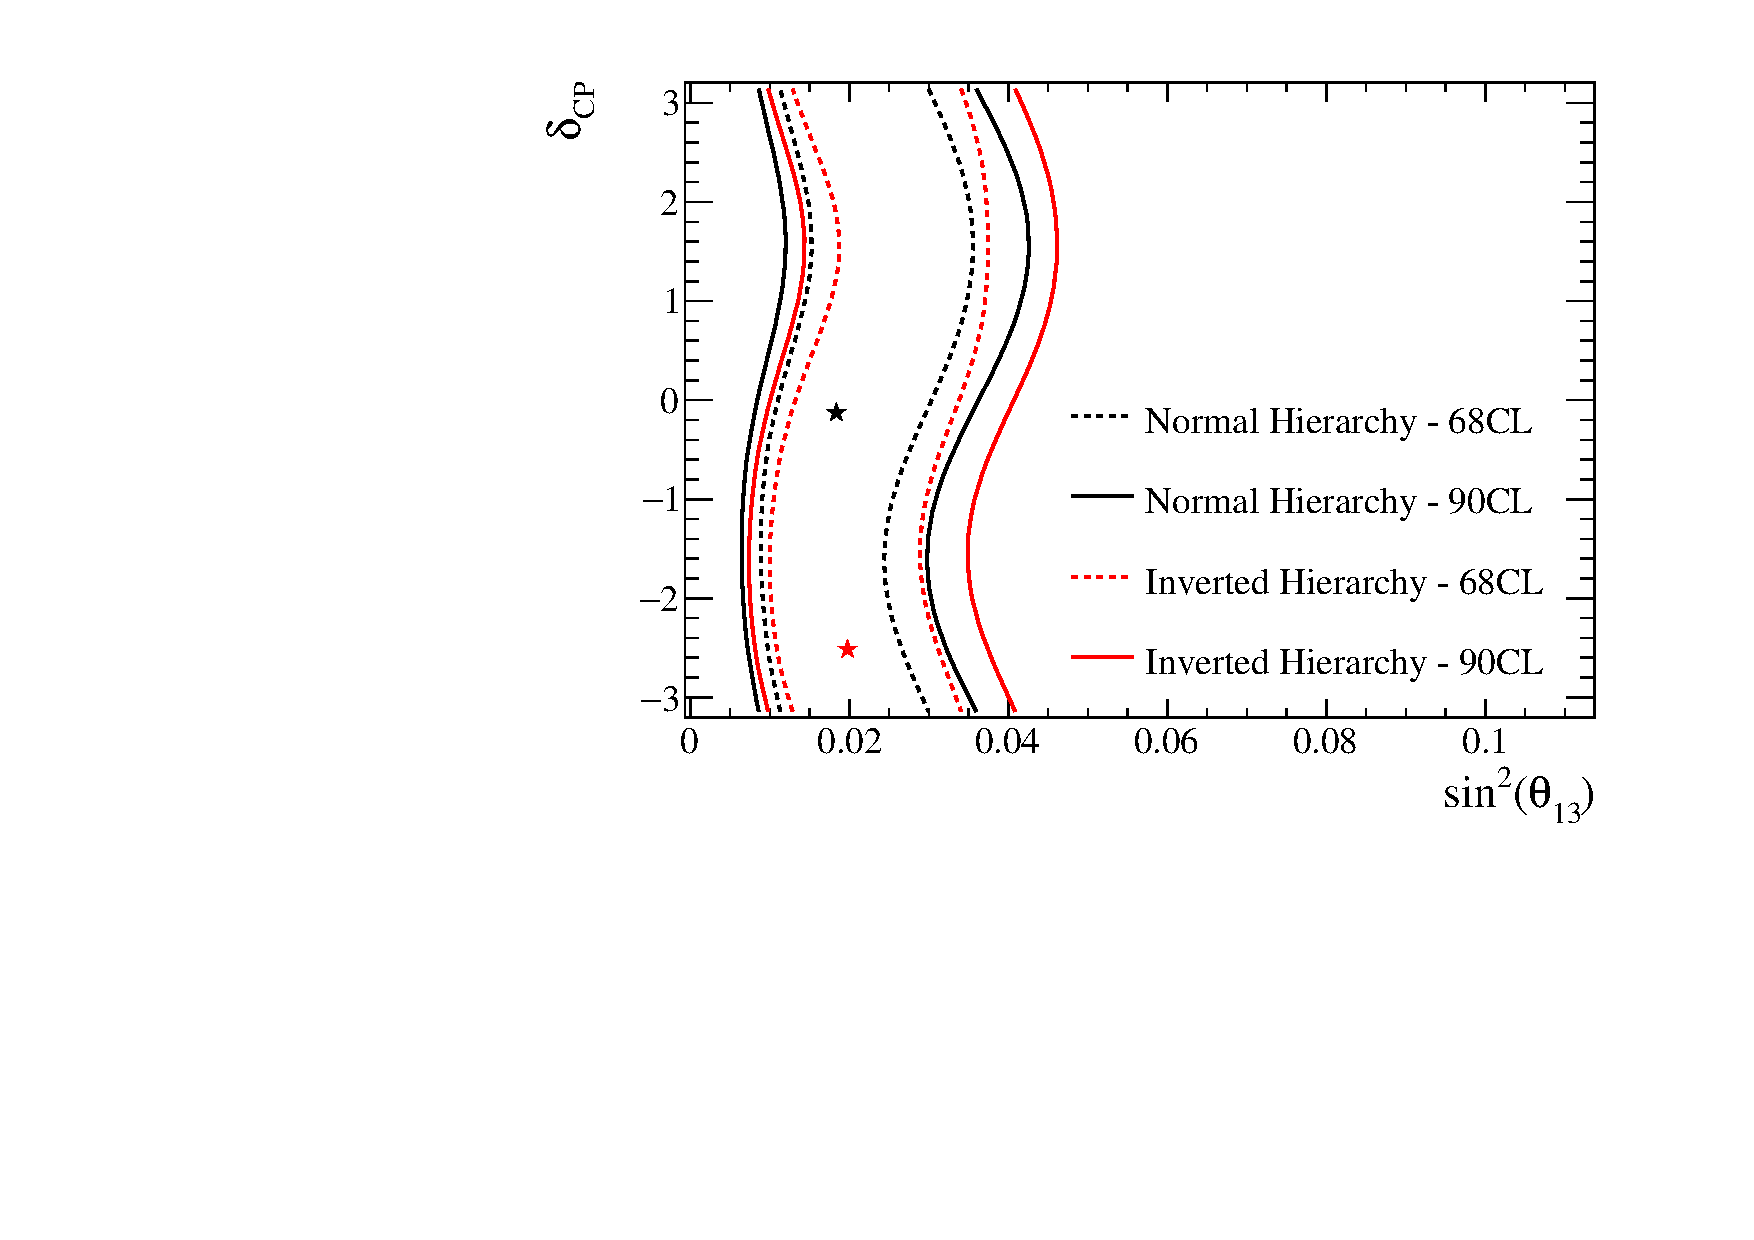
\includegraphics[width=0.9\textwidth]{./joint_plots/sensitivities/2D/cp13/cp13_B.pdf}
\caption{Asimov B with reactor constraint}
\end{subfigure}

%\begin{subfigure}[b]{0.49\textwidth}
%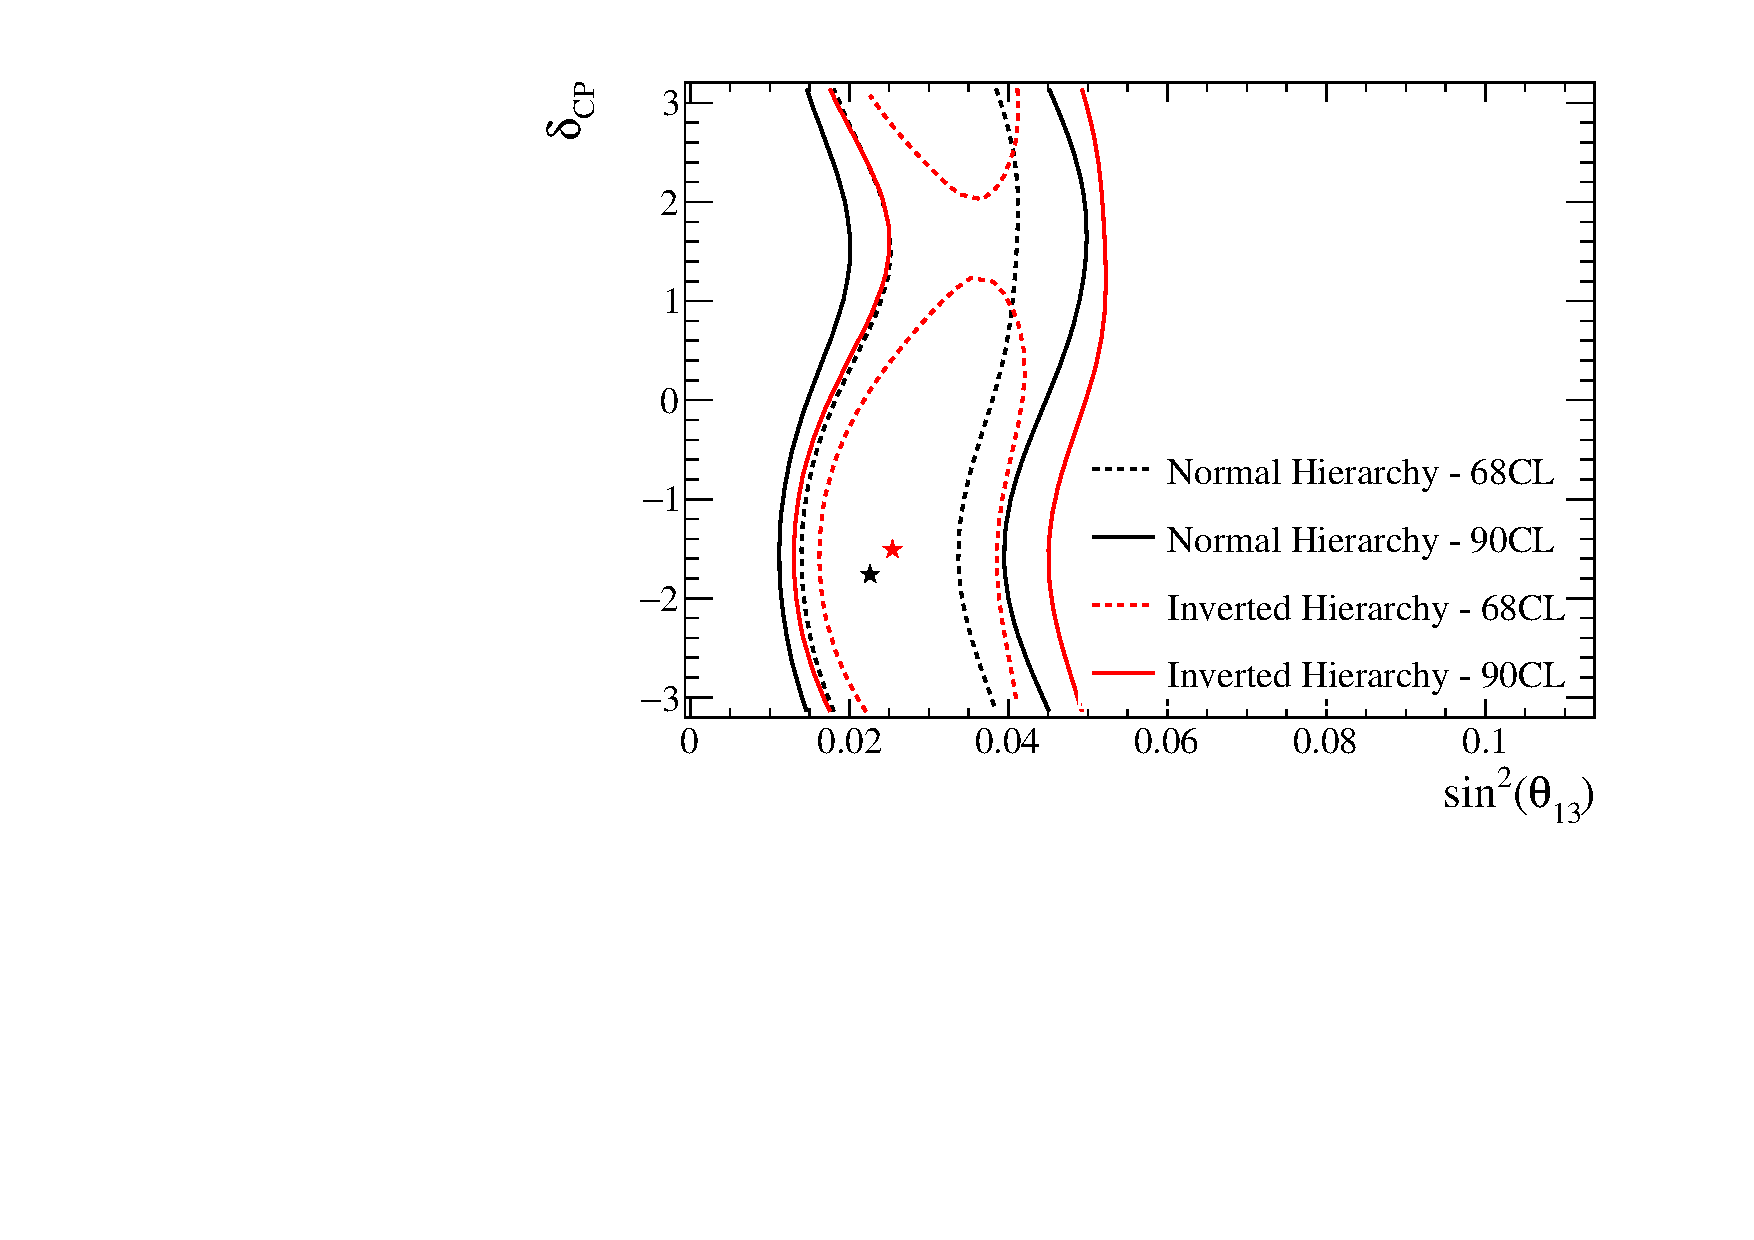
\includegraphics[width=0.9\textwidth]{./joint_plots/sensitivities/2D/cp13/cp13_A.pdf}
%\caption{Asimov A T2K only}
%\end{subfigure}
%\begin{subfigure}[b]{0.49\textwidth}
%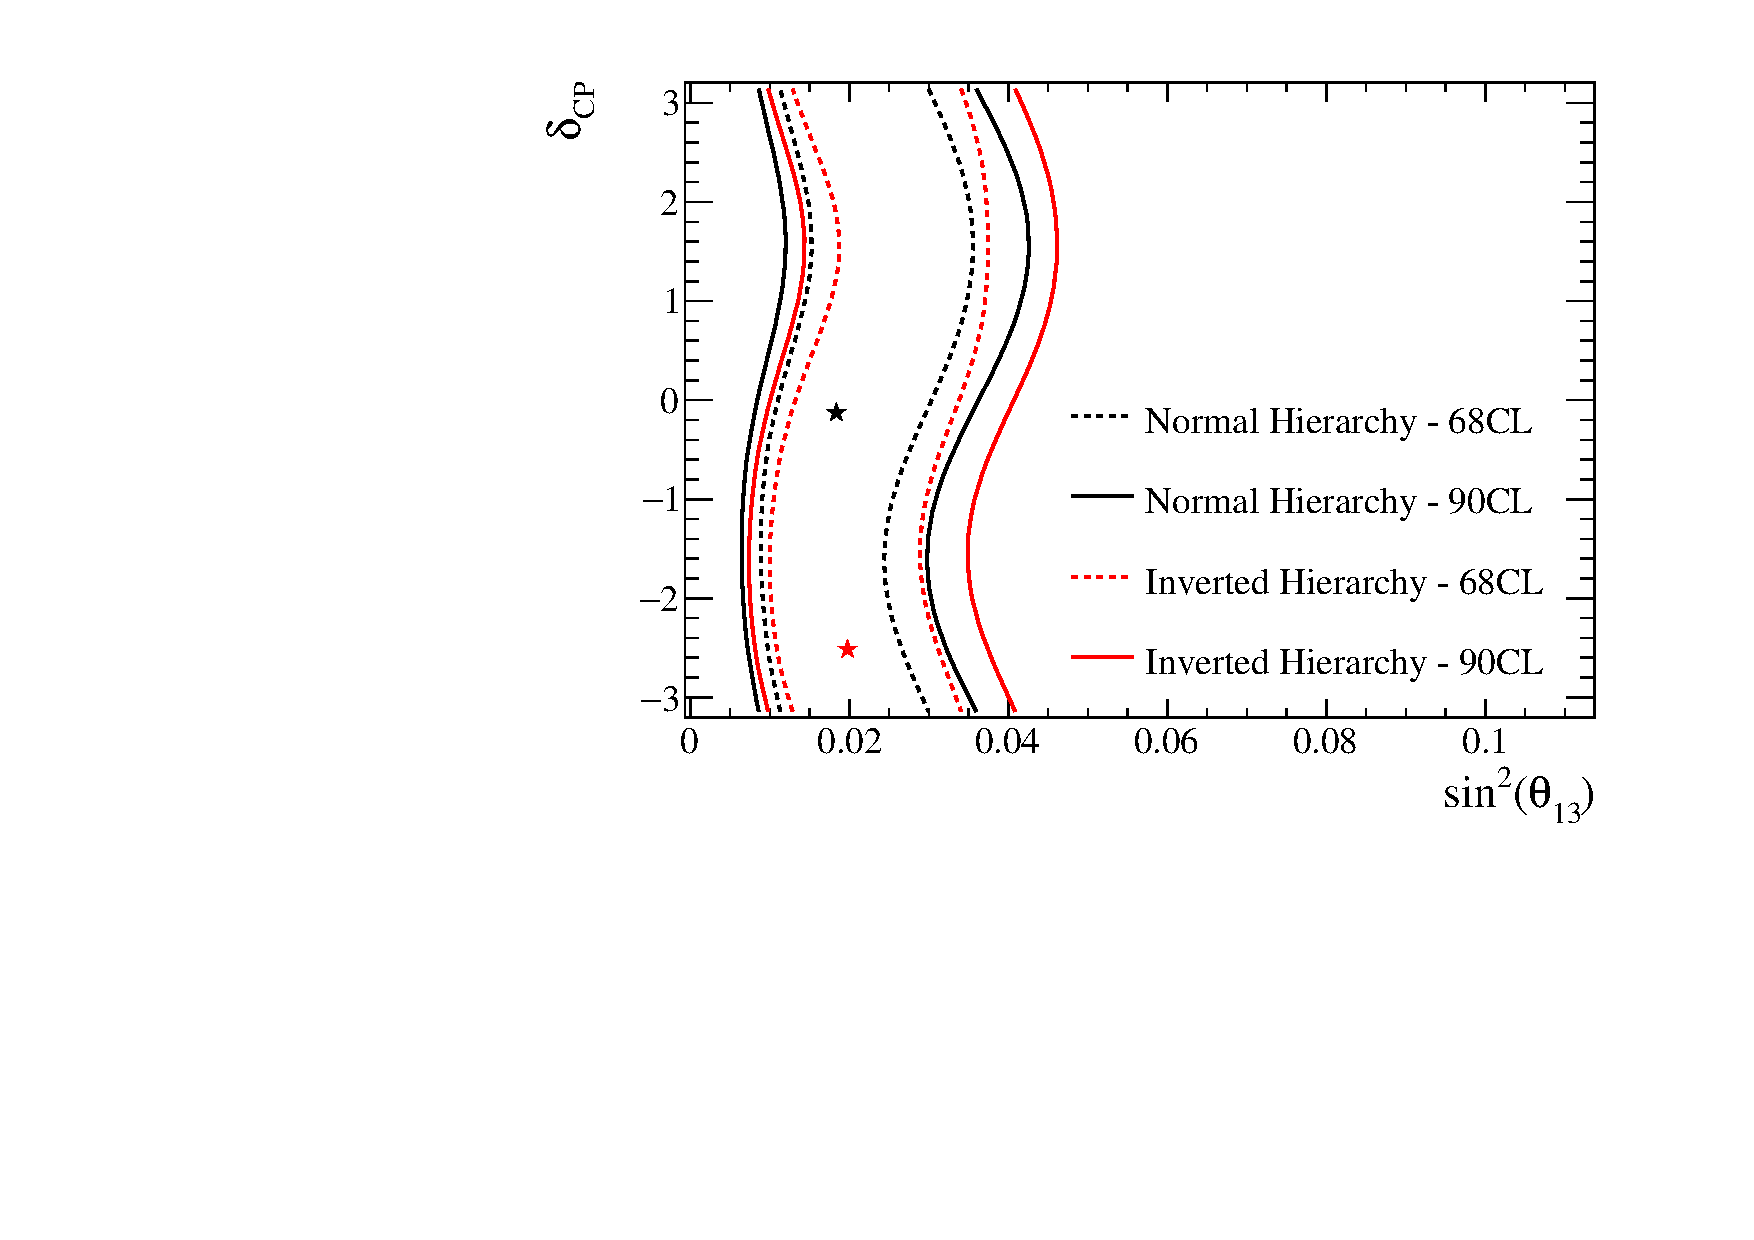
\includegraphics[width=0.9\textwidth]{./joint_plots/sensitivities/2D/cp13/cp13_B.pdf}
%\caption{Asimov B T2K only}
%\end{subfigure}

%\includegraphics[width=0.9\textwidth]{./joint_plots/sensitivities/2D/}
%\includegraphics[width=0.9\textwidth]{./joint_plots/sensitivities/2D/} \\
%\includegraphics[width=0.9\textwidth]{./joint_plots/sensitivities/2D/}
%\includegraphics[width=0.9\textwidth]{./joint_plots/sensitivities/2D/}
\caption {
%{\large{SENSI 2D CONTOURS W/ AND W/O REACTORS}}
The contours at 68\% and 90\% CL for $\sin^2 \theta_{13}$ Vs $\delta_{CP}$
for the Asimov data sets A and B of tab.~\ref{tab:osc_params_joint_asimov} 
corresponding to the Run 1-6 statistics 
is shown.
%is compared to the result obtained by the other analysis groups.
Normal and inverted hierarchy contours are independent.
}
\label{fig:validation_sensi_2d_t2konly}
\end{figure*}

%In Fig.~\ref{fig:validation_data_run14_1d} and~\ref{fig:validation_data_run14_2d} 
%the same $\Delta \chi^2$ distributions for $\delta_{CP}$ 
%as well as the same contours are 
%shown for the Run 1-4 data set and compared to the other analysis groups results.
%
%\begin{figure*}[htb]
%\center
%
\includegraphics[width=0.9\textwidth]{./images/missing_plot-eps-converted-to.pdf}
%
\includegraphics[width=0.9\textwidth]{./images/missing_plot-eps-converted-to.pdf}
%\caption {
%{\large{RUN14 DELTACHISQ 1D DELTACP W/ AND W/O REACTORS}}
%The $\Delta \chi^2$ distribution as a function of $\delta_{CP}$ 
%with reactor constraint (left) and T2K only data (right) 
%for the Run 1-4 data set
%is compared to the result obtained by the other analysis groups.
%The mass hierarchy is minimized:
%both the normal and inverted hierarchy $\chi^2$ distributions 
%are shifted to the same global best-fit $\chi^2$ value,
%which is taken as the minimum between normal and inverted hierarchy.
%}
%\label{fig:validation_data_run14_1d}
%\end{figure*}
%
%\begin{figure*}[htb]
%\center
%
\includegraphics[width=0.9\textwidth]{./images/missing_plot-eps-converted-to.pdf}
%
\includegraphics[width=0.9\textwidth]{./images/missing_plot-eps-converted-to.pdf}
%
\includegraphics[width=0.9\textwidth]{./images/missing_plot-eps-converted-to.pdf}
%\caption {
%{\large{RUN14 2D CONTOURS W/ AND W/O REACTORS}}
%The contours at 68\% and 90\% CL 
%of $\sin^2 \theta_{13}$ Vs $\delta_{CP}$ 
%with reactor constraint (top left) and T2K only data (top right)
%and
%$\sin^2 \theta_{23}$ Vs $|\Delta m^2_{32}|$ 
%with reactor constraint (bottom left) and T2K only data (bottom right)
%for the Run 1-4 data set of tab.~\ref{tab:osc_params_joint} 
%is compared to the result obtained by the other analysis groups.
%Normal and inverted hierarchy contours are independent.
%}
%\label{fig:validation_data_run14_2d}
%\end{figure*}
%
%\vspace{3mm}
%{\huge{
%TODO: ADD COMMENT ON THE SENSITIVITY COMPARISONS
%}}
%\vspace{3mm}


\clearpage



%
% Coverage study of deltaCP
% 

\subsection{Coverage study of $\delta_{CP}$}
\label{sec:coverage_deltacp}

The fit validation is performed also by making coverage studies for the fit of 
the mass hierarchy (MH) and $\delta_{CP}$ with the reactor constraint, which is the main 
result of this release of the $\bar{\nu}/\nu$ joint fit,
in order to understand if the ``Feldman-Cousins method" is needed.
The coverage is defined as the number of times the true values of $\delta_{CP}^{true}$ and $\text{MH}^{true}$, used to generate the toys MC,
is contained in the confidence interval defined by eq.~\ref{eq:condition_cl}:

\begin{equation}
\Delta \chi^2 (\delta_{CP},\text{MH}) = \chi^2 (\delta_{CP}^{true},\text{MH}^{true}) - \chi^2 (\delta_{CP}^{bf},\text{MC}^{bf}) < \Delta \chi^2_{crit}
\label{eq:coverage}
\end{equation}

where $\delta_{CP}^{bf}$ and $\text{MH}^{bf}$ are the best-fit values.
Adopting the ``constant $\Delta \chi^2$" method, the critical value $\Delta \chi^2_{crit} = \Delta \chi^2_{crit}$  
at a certain $X$\% confidence level is used for any value of $\delta_{CP}$ and MH.
Many toys MC are performed (10k) and for each one eq.~\ref{eq:coverage} is tested.
The fit has a good coverage if the number of toys MC,
for which eq.~\ref{eq:coverage} is satisfied ($N_{toys}^{X}$),
is equal or close to $X$\% within the statistical uncertainty of the number of toys MC.
If the $N_{toys}^{X} > X\%$, then the fit has over-coverage,
that means the confidence intervals should be tighter than what obtained with 
the ``constant $\Delta \chi^2$ method",
while if $N_{toys}^{X} < X\%$, then the fit has under-coverage 
and excludes a wider range of values than in the correct case.
In Fig.~\ref{fig:coverage_dcp} the coverage study 
of $\delta_{CP}$ 1-dimensional fit with reactor constraint
is shown for the true values $\delta_{CP} = -\pi/2, 0, +\pi/2$
and both mass hierarchies.

\begin{figure*}[htb]
\center
\begin{subfigure}[b]{0.49\textwidth}

\includegraphics[width=0.9\textwidth]{./images/missing_plot-eps-converted-to.pdf}
\caption{$\delta_{CP}^{true} = XXX$ with reactor constraint}
\end{subfigure}
\begin{subfigure}[b]{0.49\textwidth}

\includegraphics[width=0.9\textwidth]{./images/missing_plot-eps-converted-to.pdf}
\caption{$\delta_{CP}^{true} = XXX$ with reactor constraint}
\end{subfigure}
\begin{subfigure}[b]{0.49\textwidth}

\includegraphics[width=0.9\textwidth]{./images/missing_plot-eps-converted-to.pdf}
\caption{Critical values done with the ``Feldman-Cousins" method as a function of $\delta_{CP}^{true}$,
compared with constant $\delta \chi^2$ critical values}
\end{subfigure}
\begin{subfigure}[b]{0.49\textwidth}

\includegraphics[width=0.9\textwidth]{./images/missing_plot-eps-converted-to.pdf}
\caption{Coverage as a function of $\delta_{CP}^{true}$}
\end{subfigure}
\caption {
Coverage study of $\delta_{CP}$ with reactor constraint
for the true values $\delta_{CP} = -\pi/2, 0, +\pi/2$
assuming normal hierarchy.
All the other oscillation parameters are marginalised
and the mass hierarchy is kept fixed to normal in the fit.
The statistics corresponds to the Run 1-6 data set.
}
\label{fig:coverage_dcp}
\end{figure*}

\vspace{3mm}
{\huge{
TODO: ADD COMMENT ON COVERAGE STUDY
}}
\vspace{3mm}





%%
%% Pulls study oscillation parameters
%% 
%
%\subsection{Pull study of oscillation parameters}
%\label{sec:pulls}
%
%Pull studies are performed as well 
%for 1-dimensional fits of the oscillation parameters,
%since $1\sigma$ error ranges will be provided for each one independently.
%All the other oscillation parameters are marginalised.
%Since for the current low statistics combined with the non-gaussian behaviour
%they are not expected to be gaussian with mean 0 and pull width 1, but
%to have large deviations, for most of the parameters.
%In particular this is true for $\delta_{CP}$, which is cyclic and the values $\pm \pi/2$ behave like a boundary. 
%
%The performance of the fitter was evaluated using ensembles of 5k toy MC experiments, and these were
%generated with statistical fluctuations and variations of all \NSyst{} systematic parameters.
%Toy ensembles were generated for normal hierarchy, which was kept fixed in the fit, 
%and were fitted using the implemented minimization algorithm as described in sec.~\ref{sec:marginalization}.
%
%Asymmetric errors were calculated by choosing the $\pm 1 \sigma$ error as
%the range of free parameter values that satisfy eq.~\ref{eq:coverage}
%with $\Delta \chi^2 = 1$, i.e. the critical value of the $1\sigma$ CL
%(``constant $\Delta \chi^2$ method").
%
%For a free parameter $\theta$ the pull is defined as:
%
%\begin{align}
%&\text{if}( \theta_{bf} > \theta_{true} ) ~\text{pull} = \frac{ \theta_{bf} - \theta_{true}}{\sigma^-_{bf}}  \nonumber \\
%&\text{if}( \theta_{bf} < \theta_{true} ) ~\text{pull} = \frac{ \theta_{bf} - \theta_{true}}{\sigma^+_{bf}} 
%\end{align}
%\label{eq:pull_osc}
%
%where $\sigma^+_{bf}$ is the positive best-fit error and
%$\sigma^-_{bf}$ is the negative best-fit error of $\theta$.
%
%The pull study was performed for the oscillation parameters
%$\delta_{CP}$ with reactor constraint, $\sin^2 \theta_{13}$ with T2K only data,
%$\sin^2 \theta_{23}$ with reactor constraint and $|\Delta m^2_{32}|$ with reactor constraint
%for the Asimov data set of Tab.~\ref{tab:osc_params_joint_asimov}
%and is shown in Fig.~\ref{fig:pull_osc}.
%
%\begin{figure*}[htb]
%\center
%
\includegraphics[width=0.9\textwidth]{./images/missing_plot-eps-converted-to.pdf}
%
\includegraphics[width=0.9\textwidth]{./images/missing_plot-eps-converted-to.pdf}
%
\includegraphics[width=0.9\textwidth]{./images/missing_plot-eps-converted-to.pdf}
%
\includegraphics[width=0.9\textwidth]{./images/missing_plot-eps-converted-to.pdf}
%\caption {
%{\large{PULLS FOR EACH OSCILLATION PARAMETER ASIMOV DATA SET}}
%Pull distributions of 
%$\delta_{CP}$ with reactor constraint, $\sin^2 \theta_{13}$ with T2K only data,
%$\sin^2 \theta_{23}$ with reactor constraint and $|\Delta m^2_{32}|$ with reactor constraint
%assuming normal hierarchy for the Asimov data set of Tab.~\ref{tab:osc_params_joint_asimov}.
%In each fit all the other oscillation parameters are marginalised
%and the mass hierarchy is kept fixed to normal in the fit.
%The statistics corresponds to the Run 1-6 data set.
%The pulls are defined as in Eq.~\ref{eq:pull_osc}.
%}
%\label{fig:pull_osc}
%\end{figure*}
%
%\vspace{3mm}
%{\huge{
%TODO: ADD COMMENT ON PULL STUDY
%}}
%\vspace{3mm}
%



\clearpage

